% Options for packages loaded elsewhere
\PassOptionsToPackage{unicode}{hyperref}
\PassOptionsToPackage{hyphens}{url}
\PassOptionsToPackage{dvipsnames,svgnames,x11names}{xcolor}
%
\documentclass[
  letterpaper,
  DIV=11,
  numbers=noendperiod]{scrartcl}

\usepackage{amsmath,amssymb}
\usepackage{lmodern}
\usepackage{iftex}
\ifPDFTeX
  \usepackage[T1]{fontenc}
  \usepackage[utf8]{inputenc}
  \usepackage{textcomp} % provide euro and other symbols
\else % if luatex or xetex
  \usepackage{unicode-math}
  \defaultfontfeatures{Scale=MatchLowercase}
  \defaultfontfeatures[\rmfamily]{Ligatures=TeX,Scale=1}
\fi
% Use upquote if available, for straight quotes in verbatim environments
\IfFileExists{upquote.sty}{\usepackage{upquote}}{}
\IfFileExists{microtype.sty}{% use microtype if available
  \usepackage[]{microtype}
  \UseMicrotypeSet[protrusion]{basicmath} % disable protrusion for tt fonts
}{}
\makeatletter
\@ifundefined{KOMAClassName}{% if non-KOMA class
  \IfFileExists{parskip.sty}{%
    \usepackage{parskip}
  }{% else
    \setlength{\parindent}{0pt}
    \setlength{\parskip}{6pt plus 2pt minus 1pt}}
}{% if KOMA class
  \KOMAoptions{parskip=half}}
\makeatother
\usepackage{xcolor}
\setlength{\emergencystretch}{3em} % prevent overfull lines
\setcounter{secnumdepth}{-\maxdimen} % remove section numbering
% Make \paragraph and \subparagraph free-standing
\ifx\paragraph\undefined\else
  \let\oldparagraph\paragraph
  \renewcommand{\paragraph}[1]{\oldparagraph{#1}\mbox{}}
\fi
\ifx\subparagraph\undefined\else
  \let\oldsubparagraph\subparagraph
  \renewcommand{\subparagraph}[1]{\oldsubparagraph{#1}\mbox{}}
\fi

\usepackage{color}
\usepackage{fancyvrb}
\newcommand{\VerbBar}{|}
\newcommand{\VERB}{\Verb[commandchars=\\\{\}]}
\DefineVerbatimEnvironment{Highlighting}{Verbatim}{commandchars=\\\{\}}
% Add ',fontsize=\small' for more characters per line
\usepackage{framed}
\definecolor{shadecolor}{RGB}{241,243,245}
\newenvironment{Shaded}{\begin{snugshade}}{\end{snugshade}}
\newcommand{\AlertTok}[1]{\textcolor[rgb]{0.68,0.00,0.00}{#1}}
\newcommand{\AnnotationTok}[1]{\textcolor[rgb]{0.37,0.37,0.37}{#1}}
\newcommand{\AttributeTok}[1]{\textcolor[rgb]{0.40,0.45,0.13}{#1}}
\newcommand{\BaseNTok}[1]{\textcolor[rgb]{0.68,0.00,0.00}{#1}}
\newcommand{\BuiltInTok}[1]{\textcolor[rgb]{0.00,0.23,0.31}{#1}}
\newcommand{\CharTok}[1]{\textcolor[rgb]{0.13,0.47,0.30}{#1}}
\newcommand{\CommentTok}[1]{\textcolor[rgb]{0.37,0.37,0.37}{#1}}
\newcommand{\CommentVarTok}[1]{\textcolor[rgb]{0.37,0.37,0.37}{\textit{#1}}}
\newcommand{\ConstantTok}[1]{\textcolor[rgb]{0.56,0.35,0.01}{#1}}
\newcommand{\ControlFlowTok}[1]{\textcolor[rgb]{0.00,0.23,0.31}{#1}}
\newcommand{\DataTypeTok}[1]{\textcolor[rgb]{0.68,0.00,0.00}{#1}}
\newcommand{\DecValTok}[1]{\textcolor[rgb]{0.68,0.00,0.00}{#1}}
\newcommand{\DocumentationTok}[1]{\textcolor[rgb]{0.37,0.37,0.37}{\textit{#1}}}
\newcommand{\ErrorTok}[1]{\textcolor[rgb]{0.68,0.00,0.00}{#1}}
\newcommand{\ExtensionTok}[1]{\textcolor[rgb]{0.00,0.23,0.31}{#1}}
\newcommand{\FloatTok}[1]{\textcolor[rgb]{0.68,0.00,0.00}{#1}}
\newcommand{\FunctionTok}[1]{\textcolor[rgb]{0.28,0.35,0.67}{#1}}
\newcommand{\ImportTok}[1]{\textcolor[rgb]{0.00,0.46,0.62}{#1}}
\newcommand{\InformationTok}[1]{\textcolor[rgb]{0.37,0.37,0.37}{#1}}
\newcommand{\KeywordTok}[1]{\textcolor[rgb]{0.00,0.23,0.31}{#1}}
\newcommand{\NormalTok}[1]{\textcolor[rgb]{0.00,0.23,0.31}{#1}}
\newcommand{\OperatorTok}[1]{\textcolor[rgb]{0.37,0.37,0.37}{#1}}
\newcommand{\OtherTok}[1]{\textcolor[rgb]{0.00,0.23,0.31}{#1}}
\newcommand{\PreprocessorTok}[1]{\textcolor[rgb]{0.68,0.00,0.00}{#1}}
\newcommand{\RegionMarkerTok}[1]{\textcolor[rgb]{0.00,0.23,0.31}{#1}}
\newcommand{\SpecialCharTok}[1]{\textcolor[rgb]{0.37,0.37,0.37}{#1}}
\newcommand{\SpecialStringTok}[1]{\textcolor[rgb]{0.13,0.47,0.30}{#1}}
\newcommand{\StringTok}[1]{\textcolor[rgb]{0.13,0.47,0.30}{#1}}
\newcommand{\VariableTok}[1]{\textcolor[rgb]{0.07,0.07,0.07}{#1}}
\newcommand{\VerbatimStringTok}[1]{\textcolor[rgb]{0.13,0.47,0.30}{#1}}
\newcommand{\WarningTok}[1]{\textcolor[rgb]{0.37,0.37,0.37}{\textit{#1}}}

\providecommand{\tightlist}{%
  \setlength{\itemsep}{0pt}\setlength{\parskip}{0pt}}\usepackage{longtable,booktabs,array}
\usepackage{calc} % for calculating minipage widths
% Correct order of tables after \paragraph or \subparagraph
\usepackage{etoolbox}
\makeatletter
\patchcmd\longtable{\par}{\if@noskipsec\mbox{}\fi\par}{}{}
\makeatother
% Allow footnotes in longtable head/foot
\IfFileExists{footnotehyper.sty}{\usepackage{footnotehyper}}{\usepackage{footnote}}
\makesavenoteenv{longtable}
\usepackage{graphicx}
\makeatletter
\def\maxwidth{\ifdim\Gin@nat@width>\linewidth\linewidth\else\Gin@nat@width\fi}
\def\maxheight{\ifdim\Gin@nat@height>\textheight\textheight\else\Gin@nat@height\fi}
\makeatother
% Scale images if necessary, so that they will not overflow the page
% margins by default, and it is still possible to overwrite the defaults
% using explicit options in \includegraphics[width, height, ...]{}
\setkeys{Gin}{width=\maxwidth,height=\maxheight,keepaspectratio}
% Set default figure placement to htbp
\makeatletter
\def\fps@figure{htbp}
\makeatother

\KOMAoption{captions}{tableheading}
\makeatletter
\makeatother
\makeatletter
\makeatother
\makeatletter
\@ifpackageloaded{caption}{}{\usepackage{caption}}
\AtBeginDocument{%
\ifdefined\contentsname
  \renewcommand*\contentsname{Table of contents}
\else
  \newcommand\contentsname{Table of contents}
\fi
\ifdefined\listfigurename
  \renewcommand*\listfigurename{List of Figures}
\else
  \newcommand\listfigurename{List of Figures}
\fi
\ifdefined\listtablename
  \renewcommand*\listtablename{List of Tables}
\else
  \newcommand\listtablename{List of Tables}
\fi
\ifdefined\figurename
  \renewcommand*\figurename{Figure}
\else
  \newcommand\figurename{Figure}
\fi
\ifdefined\tablename
  \renewcommand*\tablename{Table}
\else
  \newcommand\tablename{Table}
\fi
}
\@ifpackageloaded{float}{}{\usepackage{float}}
\floatstyle{ruled}
\@ifundefined{c@chapter}{\newfloat{codelisting}{h}{lop}}{\newfloat{codelisting}{h}{lop}[chapter]}
\floatname{codelisting}{Listing}
\newcommand*\listoflistings{\listof{codelisting}{List of Listings}}
\makeatother
\makeatletter
\@ifpackageloaded{caption}{}{\usepackage{caption}}
\@ifpackageloaded{subcaption}{}{\usepackage{subcaption}}
\makeatother
\makeatletter
\@ifpackageloaded{tcolorbox}{}{\usepackage[many]{tcolorbox}}
\makeatother
\makeatletter
\@ifundefined{shadecolor}{\definecolor{shadecolor}{rgb}{.97, .97, .97}}
\makeatother
\makeatletter
\makeatother
\ifLuaTeX
  \usepackage{selnolig}  % disable illegal ligatures
\fi
\IfFileExists{bookmark.sty}{\usepackage{bookmark}}{\usepackage{hyperref}}
\IfFileExists{xurl.sty}{\usepackage{xurl}}{} % add URL line breaks if available
\urlstyle{same} % disable monospaced font for URLs
\hypersetup{
  pdftitle={Forecasting in R},
  pdfauthor={Zahid Asghar and     Tayyaba Batool,Capacity Analytics, Islamabad},
  colorlinks=true,
  linkcolor={blue},
  filecolor={Maroon},
  citecolor={Blue},
  urlcolor={Blue},
  pdfcreator={LaTeX via pandoc}}

\title{Forecasting in R}
\author{\emph{Zahid Asghar and Tayyaba Batool,Capacity Analytics,
Islamabad}}
\date{26 September 2022}

\begin{document}
\maketitle
\ifdefined\Shaded\renewenvironment{Shaded}{\begin{tcolorbox}[sharp corners, frame hidden, borderline west={3pt}{0pt}{shadecolor}, interior hidden, enhanced, breakable, boxrule=0pt]}{\end{tcolorbox}}\fi

\renewcommand*\contentsname{Table of contents}
{
\hypersetup{linkcolor=}
\setcounter{tocdepth}{3}
\tableofcontents
}
\hypertarget{forecasting-in-r}{%
\subsection{Forecasting in R}\label{forecasting-in-r}}

\begin{Shaded}
\begin{Highlighting}[]
\FunctionTok{library}\NormalTok{(readxl)}
\CommentTok{\# Read the data from Excel into R}
\NormalTok{mydata }\OtherTok{\textless{}{-}} \FunctionTok{read\_excel}\NormalTok{(}\StringTok{"exercise1.xlsx"}\NormalTok{)}

\CommentTok{\# Look at the first few lines of mydata}
\FunctionTok{head}\NormalTok{(mydata)}

\CommentTok{\# Create a ts object called myts}
\NormalTok{myts }\OtherTok{\textless{}{-}} \FunctionTok{ts}\NormalTok{(mydata[,}\DecValTok{2}\SpecialCharTok{:}\DecValTok{4}\NormalTok{], }\AttributeTok{start =} \FunctionTok{c}\NormalTok{(}\DecValTok{1981}\NormalTok{, }\DecValTok{1}\NormalTok{), }\AttributeTok{frequency =} \DecValTok{4}\NormalTok{)}
\end{Highlighting}
\end{Shaded}

\begin{itemize}
\item
  lot the data you stored as \texttt{myts} using \texttt{autoplot()}
  with facetting.
\item
  Plot the same data without facetting by setting the appropriate
  argument to \texttt{FALSE}. What happens?
\item
  Plot the \texttt{gold}, \texttt{woolyrnq}, and \texttt{gas} time
  series in separate plots.
\item
  Use \texttt{which.max()} to spot the outlier in the \texttt{gold}
  series. Which observation was it?
\item
  Apply the \texttt{frequency()} function to each commodity to get the
  number of observations per unit time. This would return 52 for weekly
  data, for example.
\end{itemize}

\begin{Shaded}
\begin{Highlighting}[]
\FunctionTok{library}\NormalTok{(fpp2)}
\end{Highlighting}
\end{Shaded}

\begin{verbatim}
Registered S3 method overwritten by 'quantmod':
  method            from
  as.zoo.data.frame zoo 
\end{verbatim}

\begin{verbatim}
-- Attaching packages ---------------------------------------------- fpp2 2.4 --
\end{verbatim}

\begin{verbatim}
v ggplot2   3.3.6     v fma       2.4  
v forecast  8.16      v expsmooth 2.3  
\end{verbatim}

\begin{verbatim}
\end{verbatim}

\begin{Shaded}
\begin{Highlighting}[]
\FunctionTok{library}\NormalTok{(fpp3)}
\end{Highlighting}
\end{Shaded}

\begin{verbatim}
-- Attaching packages -------------------------------------------- fpp3 0.4.0 --
\end{verbatim}

\begin{verbatim}
v tibble      3.1.7     v tsibble     1.1.1
v dplyr       1.0.9     v tsibbledata 0.4.0
v tidyr       1.2.0     v feasts      0.2.2
v lubridate   1.8.0     v fable       0.3.1
\end{verbatim}

\begin{verbatim}
-- Conflicts ------------------------------------------------- fpp3_conflicts --
x lubridate::date()      masks base::date()
x dplyr::filter()        masks stats::filter()
x fabletools::forecast() masks forecast::forecast()
x tsibble::intersect()   masks base::intersect()
x tsibble::interval()    masks lubridate::interval()
x dplyr::lag()           masks stats::lag()
x tsibble::setdiff()     masks base::setdiff()
x tsibble::union()       masks base::union()
\end{verbatim}

\begin{verbatim}

Attaching package: 'fpp3'
\end{verbatim}

\begin{verbatim}
The following object is masked from 'package:fpp2':

    insurance
\end{verbatim}

\begin{Shaded}
\begin{Highlighting}[]
\CommentTok{\# Plot the data with facetting}
\CommentTok{\#autoplot(myts, facets = TRUE)}

\CommentTok{\# Plot the data without facetting}
\CommentTok{\#autoplot(myts,facets=FALSE)}

\CommentTok{\# Plot the three series}
\FunctionTok{autoplot}\NormalTok{(gold)}
\end{Highlighting}
\end{Shaded}

\begin{figure}[H]

{\centering 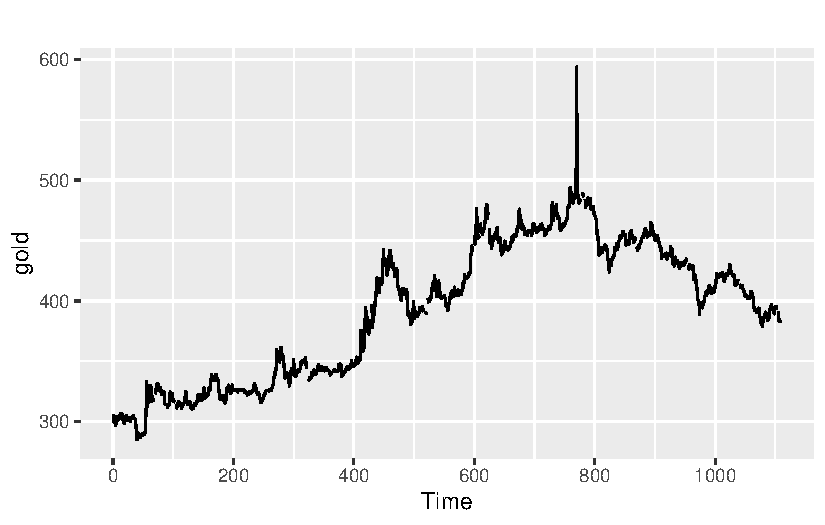
\includegraphics{forecasting_datacamp_ex_files/figure-pdf/unnamed-chunk-2-1.pdf}

}

\end{figure}

\begin{Shaded}
\begin{Highlighting}[]
\FunctionTok{autoplot}\NormalTok{(woolyrnq)}
\end{Highlighting}
\end{Shaded}

\begin{figure}[H]

{\centering 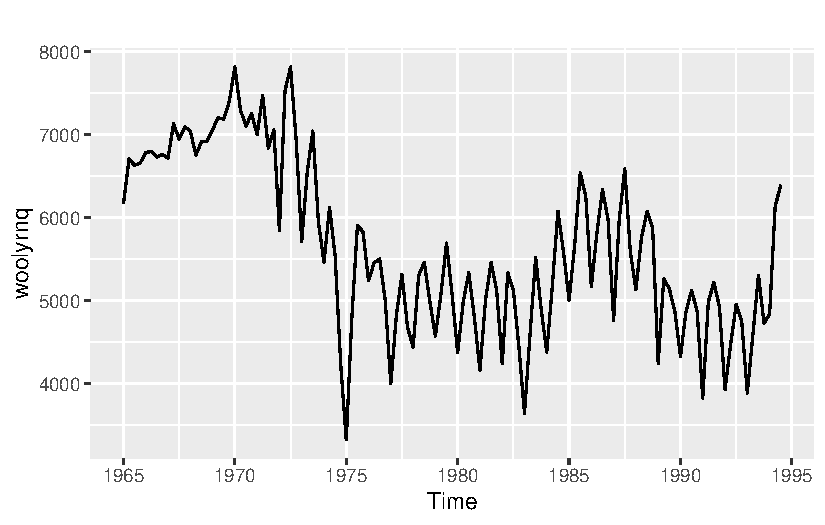
\includegraphics{forecasting_datacamp_ex_files/figure-pdf/unnamed-chunk-2-2.pdf}

}

\end{figure}

\begin{Shaded}
\begin{Highlighting}[]
\FunctionTok{autoplot}\NormalTok{(gas)}
\end{Highlighting}
\end{Shaded}

\begin{figure}[H]

{\centering 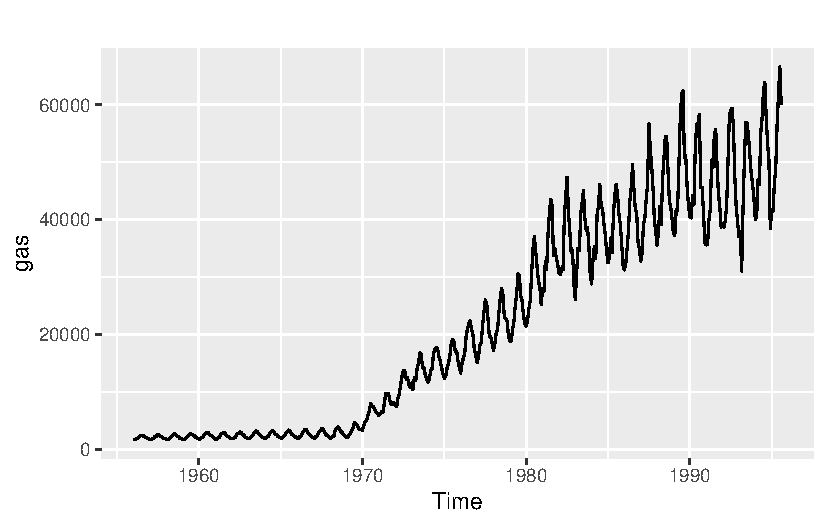
\includegraphics{forecasting_datacamp_ex_files/figure-pdf/unnamed-chunk-2-3.pdf}

}

\end{figure}

\begin{Shaded}
\begin{Highlighting}[]
\CommentTok{\# Find the outlier in the gold series}
\NormalTok{goldoutlier }\OtherTok{\textless{}{-}} \FunctionTok{which.max}\NormalTok{(gold)}

\CommentTok{\# Look at the seasonal frequencies of the three series}
\FunctionTok{frequency}\NormalTok{(gold)}
\end{Highlighting}
\end{Shaded}

\begin{verbatim}
[1] 1
\end{verbatim}

\begin{Shaded}
\begin{Highlighting}[]
\FunctionTok{frequency}\NormalTok{(woolyrnq)}
\end{Highlighting}
\end{Shaded}

\begin{verbatim}
[1] 4
\end{verbatim}

\begin{Shaded}
\begin{Highlighting}[]
\FunctionTok{frequency}\NormalTok{(gas)}
\end{Highlighting}
\end{Shaded}

\begin{verbatim}
[1] 12
\end{verbatim}

\hypertarget{seasonal-plots}{%
\subsection{Seasonal plots}\label{seasonal-plots}}

Along with time plots, there are other useful ways of plotting data to
emphasize seasonal patterns and show changes in these patterns over
time.

A seasonal plot is similar to a time plot except that the data are
plotted against the individual ``seasons'' in which the data were
observed. You can create one using the ggseasonplot() function the same
way you do with autoplot(). An interesting variant of a season plot uses
polar coordinates, where the time axis is circular rather than
horizontal; to make one, simply add a polar argument and set it to TRUE.
A subseries plot comprises mini time plots for each season. Here, the
mean for each season is shown as a blue horizontal line. One way of
splitting a time series is by using the window() function, which
extracts a subset from the object x observed between the times start and
end.

\begin{quote}
window(x, start = NULL, end = NULL) In this exercise, you will load the
fpp2 package and use two of its datasets:
\end{quote}

a10 contains monthly sales volumes for anti-diabetic drugs in Australia.
In the plots, can you see which month has the highest sales volume each
year? What is unusual about the results in March and April 2008? ausbeer
which contains quarterly beer production for Australia. What is
happening to the beer production in Quarter 4? These examples will help
you to visualize these plots and understand how they can be useful.

\hypertarget{instructions}{%
\subsubsection{Instructions}\label{instructions}}

Use library() to load the fpp2 package. Use autoplot() and
ggseasonplot() to produce plots of the a10 data. Use the ggseasonplot()
function and its polar argument to produce a polar coordinate plot for
the a10 data. Use the window() function to consider only the ausbeer
data starting from 1992. Finally, use autoplot() and ggsubseriesplot()
to produce plots of the beer series.

\begin{Shaded}
\begin{Highlighting}[]
\CommentTok{\# Load the fpp2 package}
\FunctionTok{library}\NormalTok{(fpp2)}

\CommentTok{\# Create plots of the a10 data}
\FunctionTok{autoplot}\NormalTok{(a10)}
\end{Highlighting}
\end{Shaded}

\begin{figure}[H]

{\centering 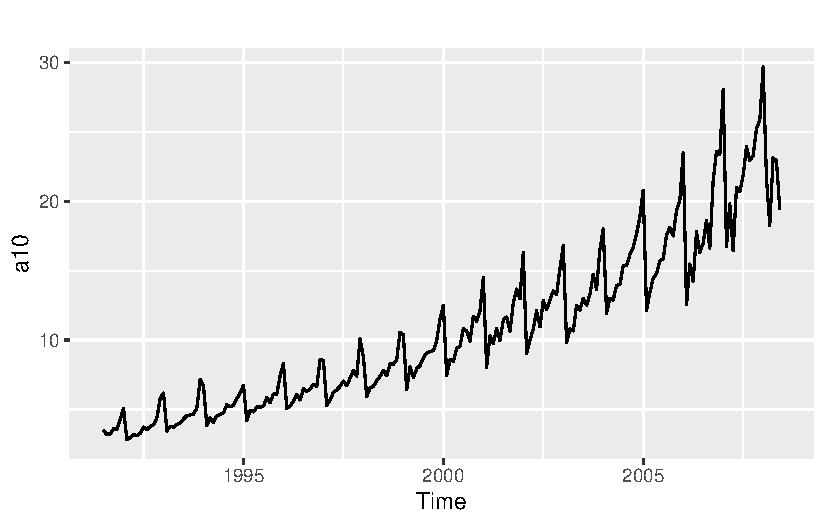
\includegraphics{forecasting_datacamp_ex_files/figure-pdf/unnamed-chunk-3-1.pdf}

}

\end{figure}

\begin{Shaded}
\begin{Highlighting}[]
\FunctionTok{ggseasonplot}\NormalTok{(a10)}
\end{Highlighting}
\end{Shaded}

\begin{figure}[H]

{\centering 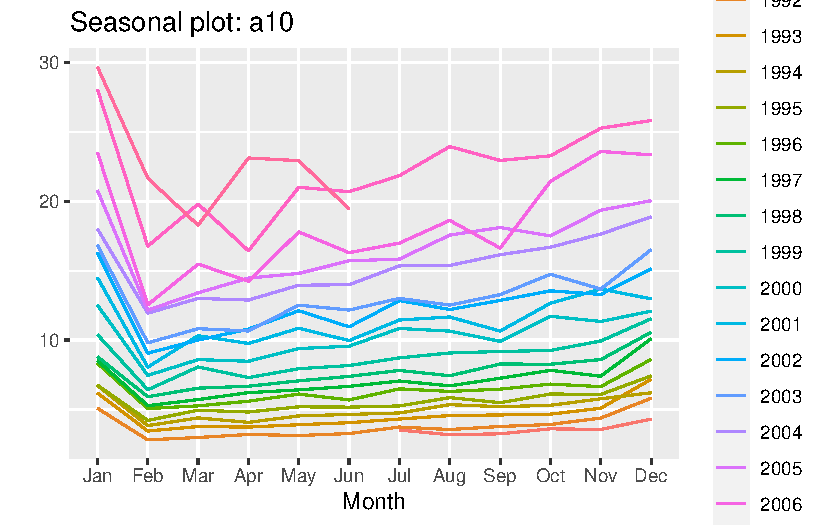
\includegraphics{forecasting_datacamp_ex_files/figure-pdf/unnamed-chunk-3-2.pdf}

}

\end{figure}

\begin{Shaded}
\begin{Highlighting}[]
\CommentTok{\# Produce a polar coordinate season plot for the a10 data}
\FunctionTok{ggseasonplot}\NormalTok{(a10, }\AttributeTok{polar =} \ConstantTok{TRUE}\NormalTok{)}
\end{Highlighting}
\end{Shaded}

\begin{figure}[H]

{\centering 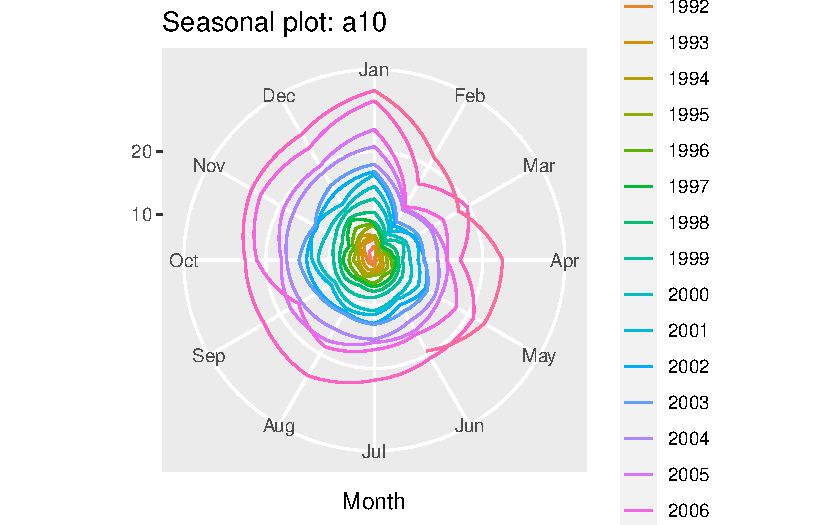
\includegraphics{forecasting_datacamp_ex_files/figure-pdf/unnamed-chunk-3-3.pdf}

}

\end{figure}

\begin{Shaded}
\begin{Highlighting}[]
\CommentTok{\# Restrict the ausbeer data to start in 1992}
\NormalTok{beer }\OtherTok{\textless{}{-}} \FunctionTok{window}\NormalTok{(ausbeer,}\AttributeTok{start=} \DecValTok{1992}\NormalTok{)}

\CommentTok{\# Make plots of the beer data}
\FunctionTok{autoplot}\NormalTok{(beer)}
\end{Highlighting}
\end{Shaded}

\begin{figure}[H]

{\centering 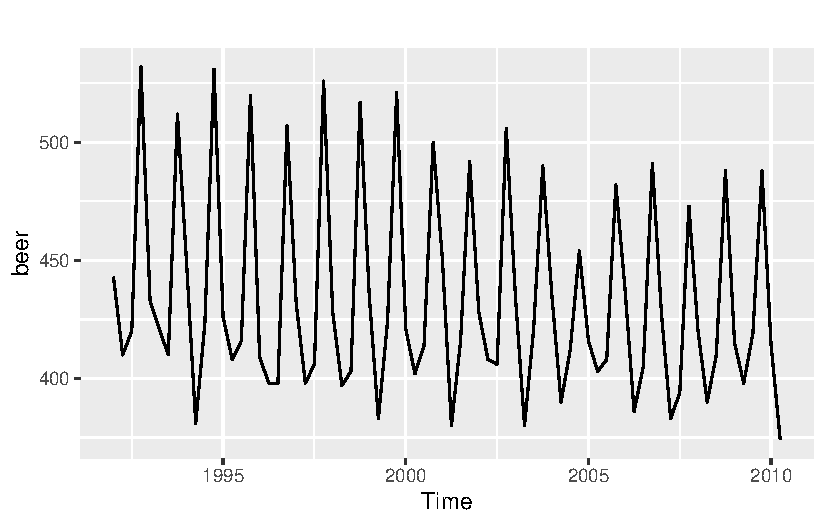
\includegraphics{forecasting_datacamp_ex_files/figure-pdf/unnamed-chunk-3-4.pdf}

}

\end{figure}

\begin{Shaded}
\begin{Highlighting}[]
\FunctionTok{ggsubseriesplot}\NormalTok{(beer)}
\end{Highlighting}
\end{Shaded}

\begin{figure}[H]

{\centering 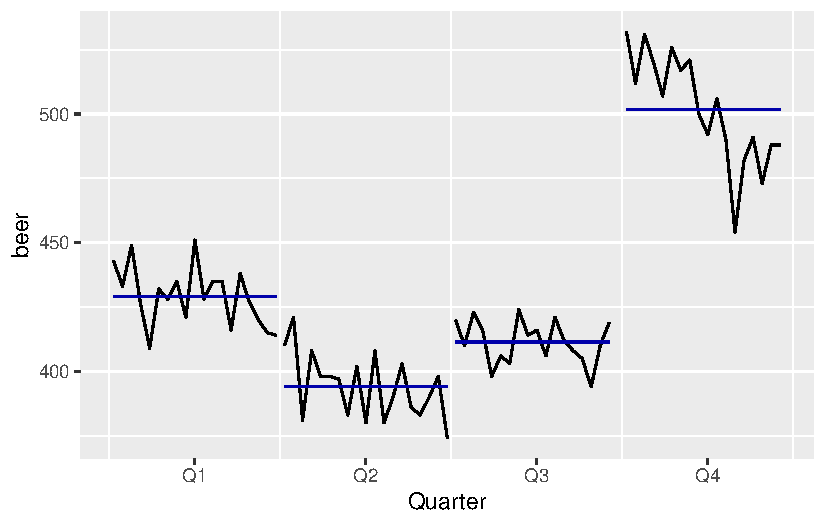
\includegraphics{forecasting_datacamp_ex_files/figure-pdf/unnamed-chunk-3-5.pdf}

}

\end{figure}

\hypertarget{autocorrelation-of-non-seasonal-time-series}{%
\subsection{Autocorrelation of non-seasonal time
series}\label{autocorrelation-of-non-seasonal-time-series}}

Another way to look at time series data is to plot each observation
against another observation that occurred some time previously by using
gglagplot(). For example, you could plot against . This is called a lag
plot because you are plotting the time series against lags of itself.

The correlations associated with the lag plots form what is called the
autocorrelation function (ACF). The ggAcf() function produces ACF plots.

In this exercise, you will work with the pre-loaded oil data (available
in the package fpp2), which contains the annual oil production in Saudi
Arabia from 1965-2013 (measured in millions of tons).

\hypertarget{instructions-1}{%
\subsubsection{Instructions}\label{instructions-1}}

Use the autoplot() function to plot the oil data. For the oil data, plot
the relationship between \(y_t\) and \(y_{t-1}, k=1,\dots,9\) using one
of the two functions introduced above. Look at how the relationships
change as the lag increases. Likewise, plot the correlations associated
with each of the lag plots using the other appropriate new function.

\begin{Shaded}
\begin{Highlighting}[]
\CommentTok{\# Create an autoplot of the oil data}
\FunctionTok{autoplot}\NormalTok{(oil)}
\end{Highlighting}
\end{Shaded}

\begin{figure}[H]

{\centering 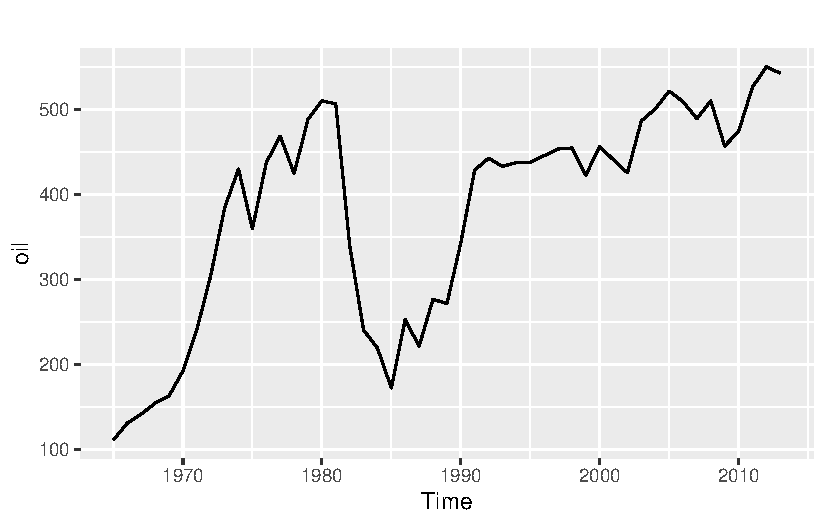
\includegraphics{forecasting_datacamp_ex_files/figure-pdf/unnamed-chunk-4-1.pdf}

}

\end{figure}

\begin{Shaded}
\begin{Highlighting}[]
\CommentTok{\# Create a lag plot of the oil data}
\FunctionTok{gglagplot}\NormalTok{(oil,}\AttributeTok{lag=}\DecValTok{1}\SpecialCharTok{:}\DecValTok{9}\NormalTok{)}
\end{Highlighting}
\end{Shaded}

\begin{verbatim}
Warning in 1:lags: numerical expression has 9 elements: only the first used
\end{verbatim}

\begin{figure}[H]

{\centering 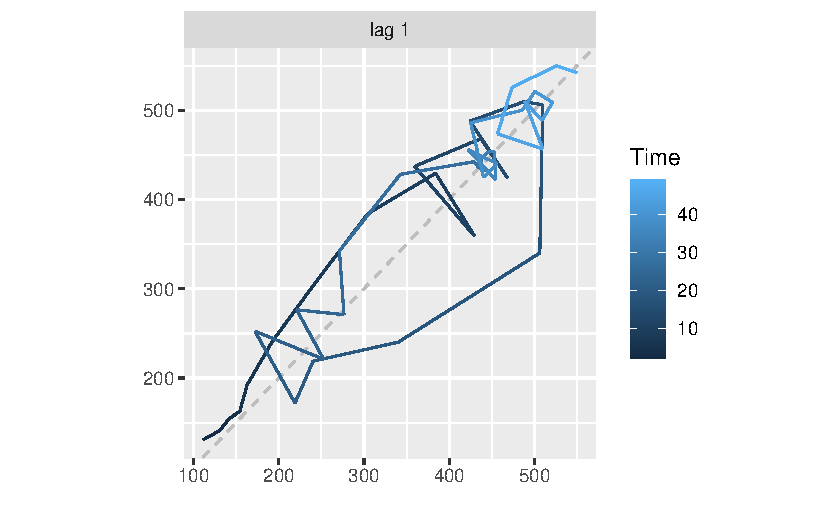
\includegraphics{forecasting_datacamp_ex_files/figure-pdf/unnamed-chunk-4-2.pdf}

}

\end{figure}

\begin{Shaded}
\begin{Highlighting}[]
\CommentTok{\# Create an ACF plot of the oil data}
\FunctionTok{ggAcf}\NormalTok{(oil)}
\end{Highlighting}
\end{Shaded}

\begin{figure}[H]

{\centering 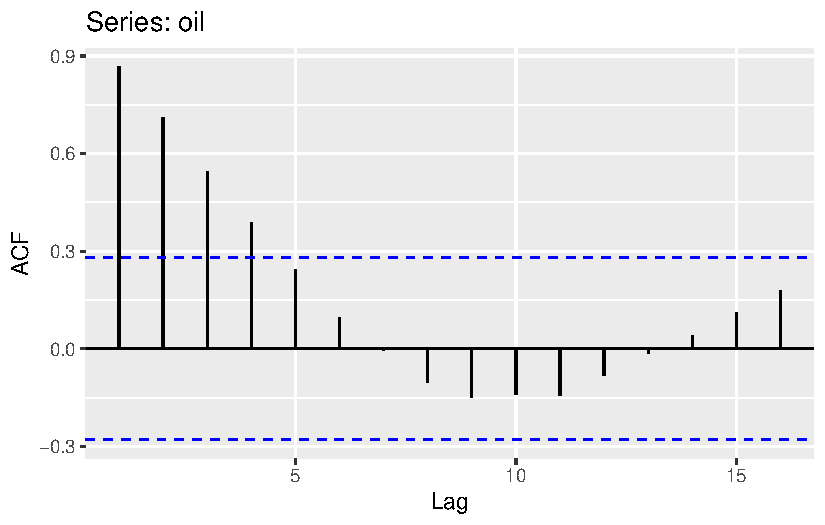
\includegraphics{forecasting_datacamp_ex_files/figure-pdf/unnamed-chunk-4-3.pdf}

}

\end{figure}

\hypertarget{autocorrelation-of-seasonal-and-cyclic-time-series}{%
\subsection{Autocorrelation of seasonal and cyclic time
series}\label{autocorrelation-of-seasonal-and-cyclic-time-series}}

When data are either seasonal or cyclic, the ACF will peak around the
seasonal lags or at the average cycle length.

You will investigate this phenomenon by plotting the annual sunspot
series (which follows the solar cycle of approximately 10-11 years) in
sunspot.year and the daily traffic to the Hyndsight blog (which follows
a 7-day weekly pattern) in hyndsight. Both objects have been loaded into
your workspace.

\hypertarget{instructions-2}{%
\subsubsection{Instructions}\label{instructions-2}}

Produce a time plot and ACF plot of sunspot.year. By observing the ACF
plot, at which lag value (x) can you find the maximum autocorrelation
(y)? Set this equal to maxlag\_sunspot. Produce a time plot and ACF plot
of hyndsight. By observing the ACF plot, at which lag value (x) can you
find the maximum autocorrelation (y)? Set this equal to
maxlag\_hyndsight.

\begin{Shaded}
\begin{Highlighting}[]
\CommentTok{\# Plot the annual sunspot numbers}
\FunctionTok{autoplot}\NormalTok{(sunspot.year)}
\end{Highlighting}
\end{Shaded}

\begin{figure}[H]

{\centering 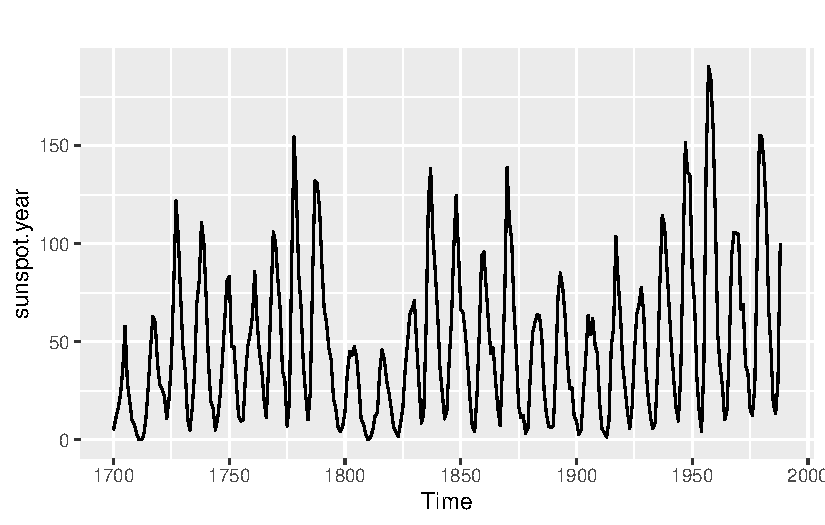
\includegraphics{forecasting_datacamp_ex_files/figure-pdf/unnamed-chunk-5-1.pdf}

}

\end{figure}

\begin{Shaded}
\begin{Highlighting}[]
\FunctionTok{ggAcf}\NormalTok{(sunspot.year)}
\end{Highlighting}
\end{Shaded}

\begin{figure}[H]

{\centering 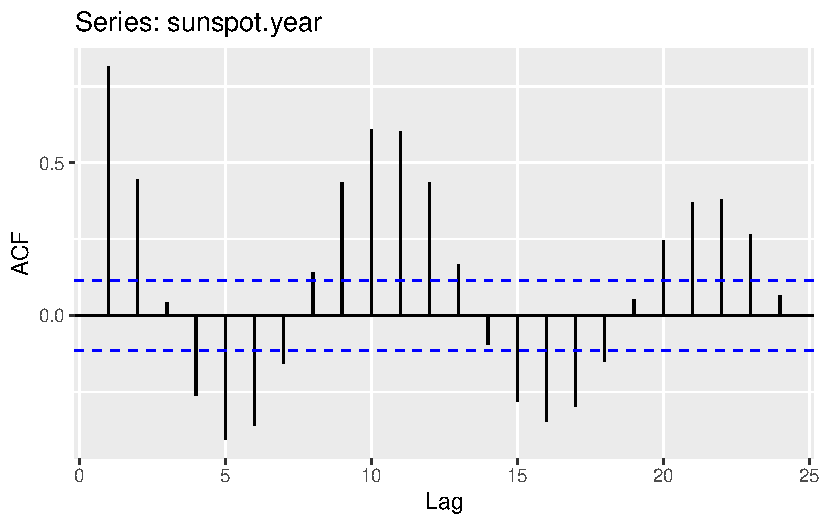
\includegraphics{forecasting_datacamp_ex_files/figure-pdf/unnamed-chunk-5-2.pdf}

}

\end{figure}

\begin{Shaded}
\begin{Highlighting}[]
\CommentTok{\# Save the lag corresponding to maximum autocorrelation}
\NormalTok{maxlag\_sunspot }\OtherTok{\textless{}{-}} \FunctionTok{lag}\NormalTok{(}\DecValTok{1}\NormalTok{)}

\CommentTok{\# Plot the traffic on the Hyndsight blog}
\FunctionTok{autoplot}\NormalTok{(hyndsight)}
\end{Highlighting}
\end{Shaded}

\begin{figure}[H]

{\centering 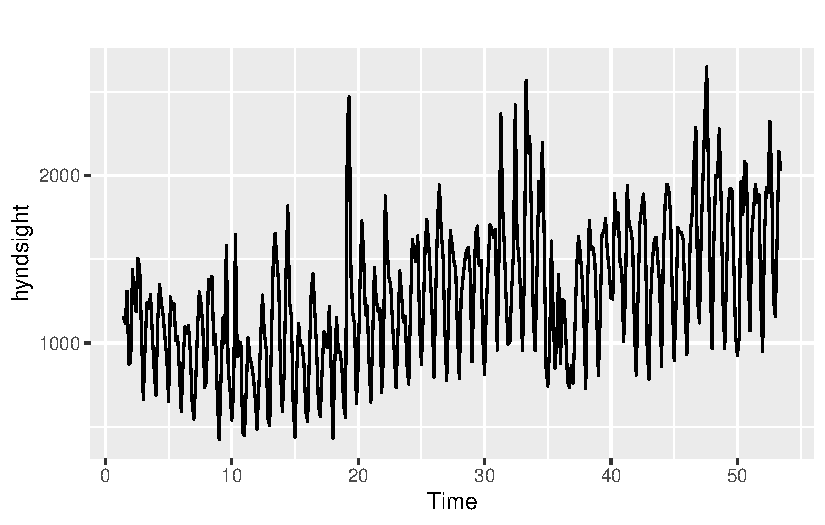
\includegraphics{forecasting_datacamp_ex_files/figure-pdf/unnamed-chunk-5-3.pdf}

}

\end{figure}

\begin{Shaded}
\begin{Highlighting}[]
\FunctionTok{ggAcf}\NormalTok{(hyndsight)}
\end{Highlighting}
\end{Shaded}

\begin{figure}[H]

{\centering 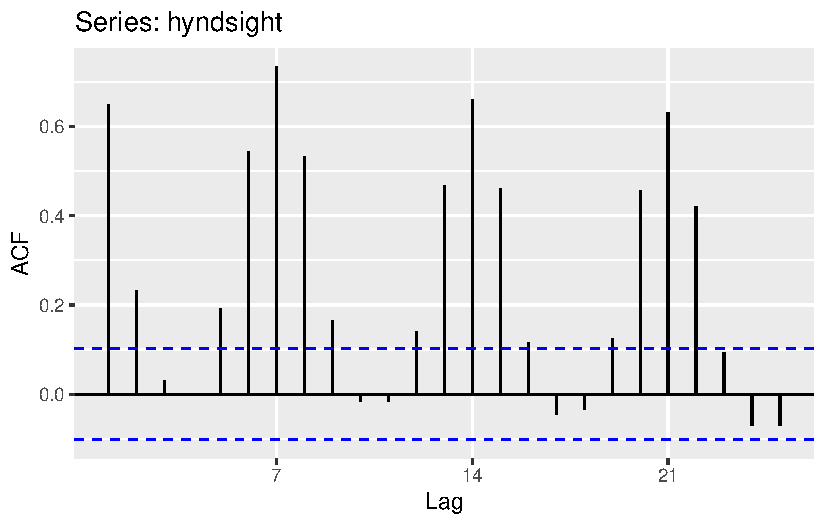
\includegraphics{forecasting_datacamp_ex_files/figure-pdf/unnamed-chunk-5-4.pdf}

}

\end{figure}

\begin{Shaded}
\begin{Highlighting}[]
\CommentTok{\# Save the lag corresponding to maximum autocorrelation}
\NormalTok{maxlag\_hyndsight }\OtherTok{\textless{}{-}} \FunctionTok{lag}\NormalTok{(}\DecValTok{7}\NormalTok{)}
\end{Highlighting}
\end{Shaded}

Possible Answers

1-B, 2-C, 3-D, 4-A

1-B, 2-A, 3-D, 4-C (correct)

1-C, 2-D, 3-B, 4-A

1-A, 2-C, 3-D, 4-B

1-C, 2-A, 3-D, 4-B

\includegraphics{series_acf.png}

\hypertarget{concept-of-white-noise-stock-market-data}{%
\subsection{Concept of white noise : Stock Market
Data}\label{concept-of-white-noise-stock-market-data}}

As you learned in the video, white noise is a term that describes purely
random data. You can conduct a Ljung-Box test using the function below
to confirm the randomness of a series; a p-value greater than 0.05
suggests that the data are not significantly different from white noise.

\begin{quote}
Box.test(pigs, lag = 24, fitdf = 0, type = ``Ljung'') There is a
well-known result in economics called the ``Efficient Market
Hypothesis'' that states that asset prices reflect all available
information. A consequence of this is that the daily changes in stock
prices should behave like white noise (ignoring dividends, interest
rates and transaction costs). The consequence for forecasters is that
the best forecast of the future price is the current price.
\end{quote}

You can test this hypothesis by looking at the goog series, which
contains the closing stock price for Google over 1000 trading days
ending on February 13, 2017. This data has been loaded into your
workspace.

\hypertarget{instructions-3}{%
\subsubsection{Instructions}\label{instructions-3}}

First plot the goog series using autoplot(). Using the diff() function
with autoplot(), plot the daily changes in Google stock prices. Use the
ggAcf() function to check if these daily changes look like white noise.
Fill in the pre-written code to do a Ljung-Box test on the daily changes
using 10 lags.

\begin{Shaded}
\begin{Highlighting}[]
\CommentTok{\# Plot the original series}
\FunctionTok{autoplot}\NormalTok{(goog)}
\end{Highlighting}
\end{Shaded}

\begin{figure}[H]

{\centering 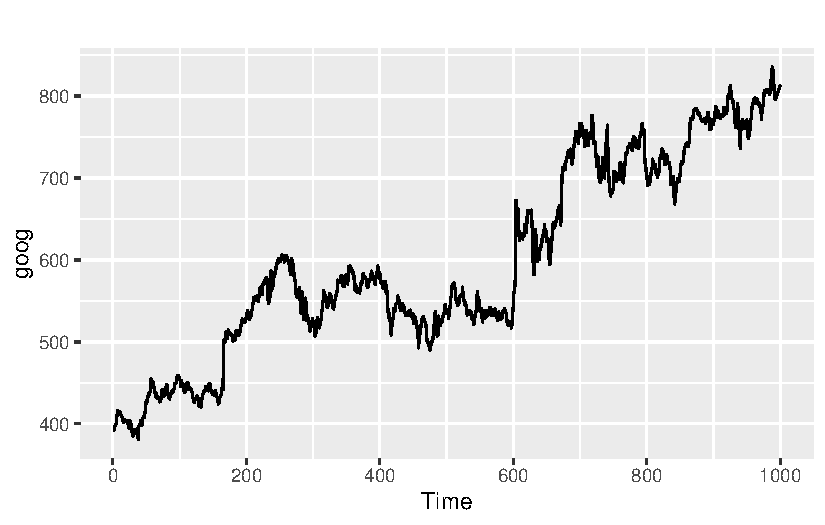
\includegraphics{forecasting_datacamp_ex_files/figure-pdf/unnamed-chunk-6-1.pdf}

}

\end{figure}

\begin{Shaded}
\begin{Highlighting}[]
\CommentTok{\# Plot the differenced series}
\FunctionTok{autoplot}\NormalTok{(}\FunctionTok{diff}\NormalTok{(goog))}
\end{Highlighting}
\end{Shaded}

\begin{figure}[H]

{\centering 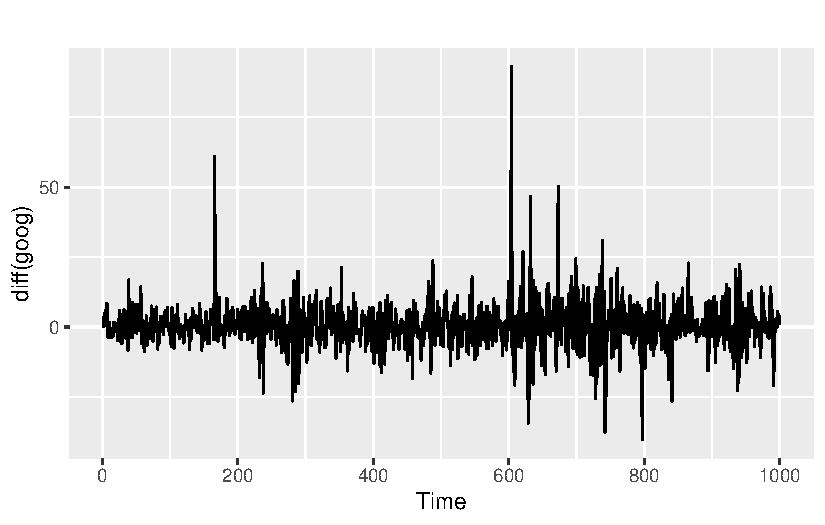
\includegraphics{forecasting_datacamp_ex_files/figure-pdf/unnamed-chunk-6-2.pdf}

}

\end{figure}

\begin{Shaded}
\begin{Highlighting}[]
\CommentTok{\# ACF of the differenced series}
\FunctionTok{ggAcf}\NormalTok{(}\FunctionTok{diff}\NormalTok{(goog))}
\end{Highlighting}
\end{Shaded}

\begin{figure}[H]

{\centering 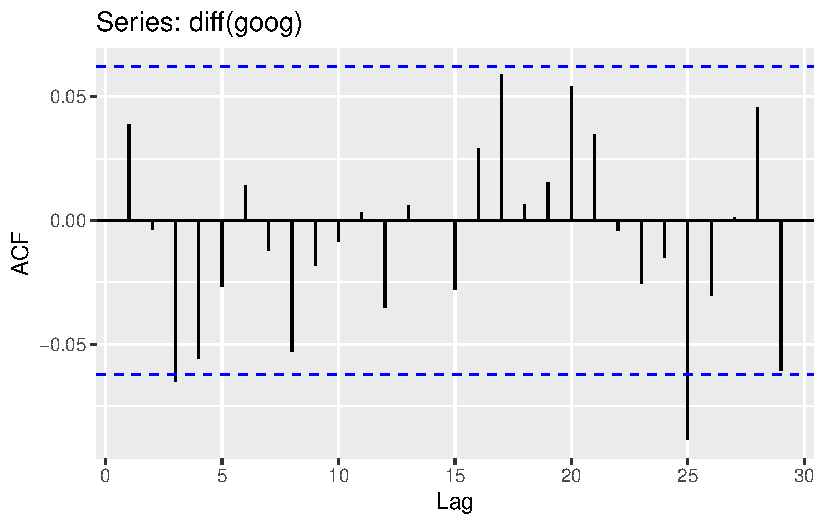
\includegraphics{forecasting_datacamp_ex_files/figure-pdf/unnamed-chunk-6-3.pdf}

}

\end{figure}

\begin{Shaded}
\begin{Highlighting}[]
\CommentTok{\# Ljung{-}Box test of the differenced series}
\FunctionTok{Box.test}\NormalTok{(}\FunctionTok{diff}\NormalTok{(goog), }\AttributeTok{lag =} \DecValTok{10}\NormalTok{, }\AttributeTok{type =} \StringTok{"Ljung"}\NormalTok{)}
\end{Highlighting}
\end{Shaded}

\begin{verbatim}

    Box-Ljung test

data:  diff(goog)
X-squared = 13.123, df = 10, p-value = 0.2169
\end{verbatim}

\hypertarget{naive-forecasting-methods}{%
\subsection{Naive forecasting methods}\label{naive-forecasting-methods}}

As you learned in the video, a forecast is the mean or median of
simulated futures of a time series.

The very simplest forecasting method is to use the most recent
observation; this is called a naive forecast and can be implemented in a
namesake function. This is the best that can be done for many time
series including most stock price data, and even if it is not a good
forecasting method, it provides a useful benchmark for other forecasting
methods.

For seasonal data, a related idea is to use the corresponding season
from the last year of data. For example, if you want to forecast the
sales volume for next March, you would use the sales volume from the
previous March. This is implemented in the snaive() function, meaning,
seasonal naive.

For both forecasting methods, you can set the second argument h, which
specifies the number of values you want to forecast; as shown in the
code below, they have different default values. The resulting output is
an object of class forecast. This is the core class of objects in the
forecast package, and there are many functions for dealing with them
including summary() and autoplot().

naive(y, h = 10) snaive(y, h = 2 * frequency(x)) You will try these two
functions on the goog series and ausbeer series, respectively. These are
available to use in your workspace.

\hypertarget{instructions-4}{%
\subsection{Instructions}\label{instructions-4}}

Use naive() to forecast the next 20 values of the goog series, and save
this to fcgoog. Plot and summarize the forecasts using autoplot() and
summary(). Use snaive() to forecast the next 16 values of the ausbeer
series, and save this to fcbeer. Plot and summarize the forecasts for
fcbeer the same way you did for fcgoog.

\begin{Shaded}
\begin{Highlighting}[]
\CommentTok{\# Use naive() to forecast the goog series}
\NormalTok{fcgoog }\OtherTok{\textless{}{-}} \FunctionTok{naive}\NormalTok{(goog,}\AttributeTok{h=}\DecValTok{20}\NormalTok{)}

\CommentTok{\# Plot and summarize the forecasts}
\FunctionTok{autoplot}\NormalTok{(fcgoog)}
\end{Highlighting}
\end{Shaded}

\begin{figure}[H]

{\centering 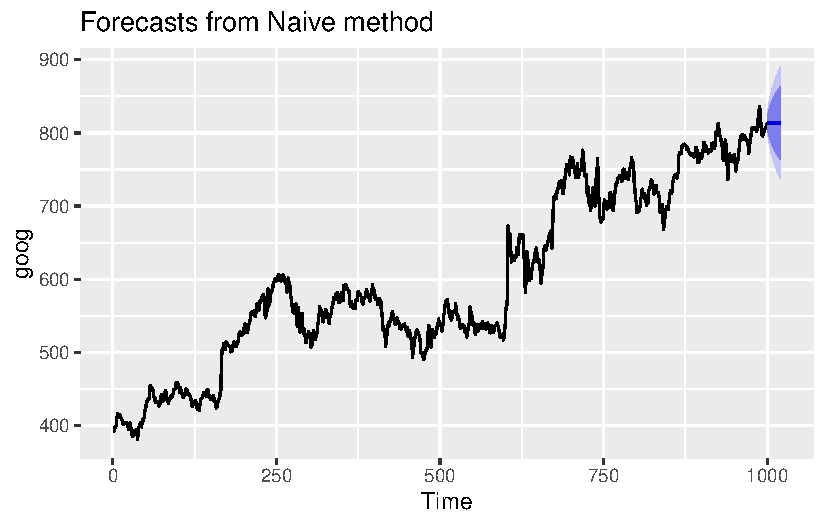
\includegraphics{forecasting_datacamp_ex_files/figure-pdf/unnamed-chunk-7-1.pdf}

}

\end{figure}

\begin{Shaded}
\begin{Highlighting}[]
\FunctionTok{summary}\NormalTok{(fcgoog)}
\end{Highlighting}
\end{Shaded}

\begin{verbatim}

Forecast method: Naive method

Model Information:
Call: naive(y = goog, h = 20) 

Residual sd: 8.7343 

Error measures:
                    ME     RMSE      MAE        MPE      MAPE MASE       ACF1
Training set 0.4212612 8.734286 5.829407 0.06253998 0.9741428    1 0.03871446

Forecasts:
     Point Forecast    Lo 80    Hi 80    Lo 95    Hi 95
1001         813.67 802.4765 824.8634 796.5511 830.7889
1002         813.67 797.8401 829.4999 789.4602 837.8797
1003         813.67 794.2824 833.0576 784.0192 843.3208
1004         813.67 791.2831 836.0569 779.4322 847.9078
1005         813.67 788.6407 838.6993 775.3910 851.9490
1006         813.67 786.2518 841.0882 771.7374 855.6025
1007         813.67 784.0549 843.2850 768.3777 858.9623
1008         813.67 782.0102 845.3298 765.2505 862.0895
1009         813.67 780.0897 847.2503 762.3133 865.0266
1010         813.67 778.2732 849.0667 759.5353 867.8047
1011         813.67 776.5456 850.7944 756.8931 870.4469
1012         813.67 774.8948 852.4452 754.3684 872.9715
1013         813.67 773.3115 854.0285 751.9470 875.3930
1014         813.67 771.7880 855.5520 749.6170 877.7230
1015         813.67 770.3180 857.0220 747.3688 879.9711
1016         813.67 768.8962 858.4437 745.1944 882.1455
1017         813.67 767.5183 859.8217 743.0870 884.2530
1018         813.67 766.1802 861.1597 741.0407 886.2993
1019         813.67 764.8789 862.4610 739.0505 888.2895
1020         813.67 763.6114 863.7286 737.1120 890.2280
\end{verbatim}

\begin{Shaded}
\begin{Highlighting}[]
\CommentTok{\# Use snaive() to forecast the ausbeer series}
\NormalTok{fcbeer }\OtherTok{\textless{}{-}} \FunctionTok{snaive}\NormalTok{(ausbeer,}\AttributeTok{h=}\DecValTok{16}\NormalTok{)}

\CommentTok{\# Plot and summarize the forecasts}
\FunctionTok{autoplot}\NormalTok{(fcbeer)}
\end{Highlighting}
\end{Shaded}

\begin{figure}[H]

{\centering 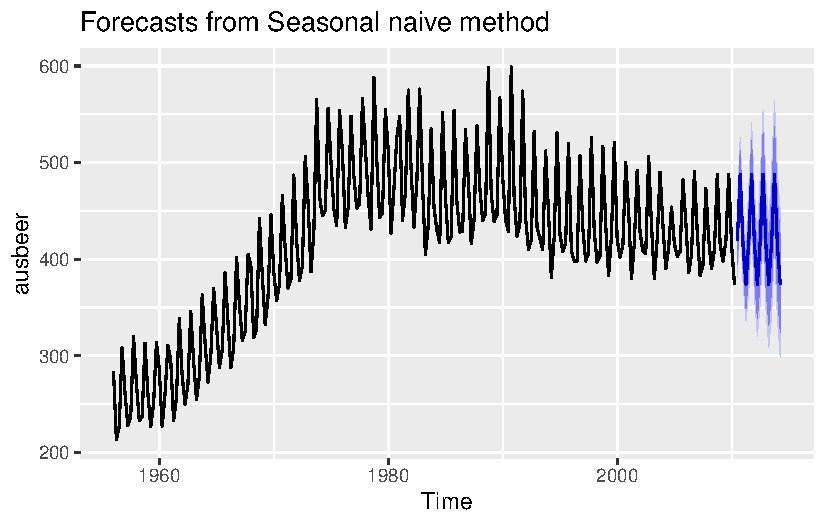
\includegraphics{forecasting_datacamp_ex_files/figure-pdf/unnamed-chunk-7-2.pdf}

}

\end{figure}

\begin{Shaded}
\begin{Highlighting}[]
\FunctionTok{summary}\NormalTok{(fcbeer)}
\end{Highlighting}
\end{Shaded}

\begin{verbatim}

Forecast method: Seasonal naive method

Model Information:
Call: snaive(y = ausbeer, h = 16) 

Residual sd: 19.3259 

Error measures:
                   ME     RMSE      MAE      MPE    MAPE MASE       ACF1
Training set 3.098131 19.32591 15.50935 0.838741 3.69567    1 0.01093868

Forecasts:
        Point Forecast    Lo 80    Hi 80    Lo 95    Hi 95
2010 Q3            419 394.2329 443.7671 381.1219 456.8781
2010 Q4            488 463.2329 512.7671 450.1219 525.8781
2011 Q1            414 389.2329 438.7671 376.1219 451.8781
2011 Q2            374 349.2329 398.7671 336.1219 411.8781
2011 Q3            419 383.9740 454.0260 365.4323 472.5677
2011 Q4            488 452.9740 523.0260 434.4323 541.5677
2012 Q1            414 378.9740 449.0260 360.4323 467.5677
2012 Q2            374 338.9740 409.0260 320.4323 427.5677
2012 Q3            419 376.1020 461.8980 353.3932 484.6068
2012 Q4            488 445.1020 530.8980 422.3932 553.6068
2013 Q1            414 371.1020 456.8980 348.3932 479.6068
2013 Q2            374 331.1020 416.8980 308.3932 439.6068
2013 Q3            419 369.4657 468.5343 343.2438 494.7562
2013 Q4            488 438.4657 537.5343 412.2438 563.7562
2014 Q1            414 364.4657 463.5343 338.2438 489.7562
2014 Q2            374 324.4657 423.5343 298.2438 449.7562
\end{verbatim}

\hypertarget{checking-time-series-residuals}{%
\subsection{Checking time series
residuals}\label{checking-time-series-residuals}}

When applying a forecasting method, it is important to always check that
the residuals are well-behaved (i.e., no outliers or patterns) and
resemble white noise. The prediction intervals are computed assuming
that the residuals are also normally distributed. You can use the
checkresiduals() function to verify these characteristics; it will give
the results of a Ljung-Box test.

You haven't used the pipe function (\%\textgreater\%) so far, but this
is a good opportunity to introduce it. When there are many nested
functions, pipe functions make the code much easier to read. To be
consistent, always follow a function with parentheses to differentiate
it from other objects, even if it has no arguments. An example is below:

\begin{quote}
function(foo) \# These two foo \%\textgreater\% function() \# are the
same!
\end{quote}

\begin{quote}
foo \%\textgreater\% function \# Inconsistent In this exercise, you will
test the above functions on the forecasts equivalent to what you
produced in the previous exercise (fcgoog obtained after applying
naive() to goog, and fcbeer obtained after applying snaive() to
ausbeer).
\end{quote}

\hypertarget{instructions-5}{%
\subsubsection{Instructions}\label{instructions-5}}

Using the above pipe function, run checkresiduals() on a forecast
equivalent to fcgoog. Based on this Ljung-Box test results, do the
residuals resemble white noise? Assign googwn to either TRUE or FALSE.
Using a similar pipe function, run checkresiduals() on a forecast
equivalent to fcbeer. Based on this Ljung-Box test results, do the
residuals resemble white noise? Assign beerwn to either TRUE or FALSE.

\begin{Shaded}
\begin{Highlighting}[]
\CommentTok{\# Check the residuals from the naive forecasts applied to the goog series}
\NormalTok{goog }\SpecialCharTok{\%\textgreater{}\%} \FunctionTok{naive}\NormalTok{() }\SpecialCharTok{\%\textgreater{}\%} \FunctionTok{checkresiduals}\NormalTok{()}
\end{Highlighting}
\end{Shaded}

\begin{figure}[H]

{\centering 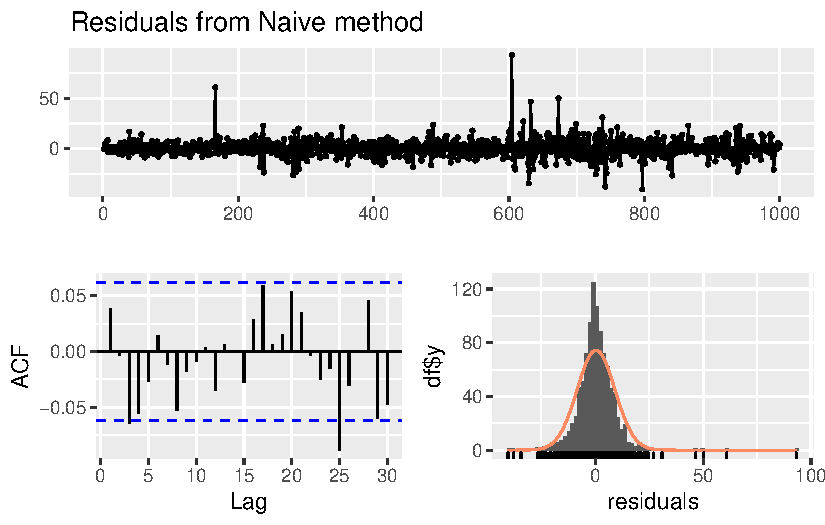
\includegraphics{forecasting_datacamp_ex_files/figure-pdf/unnamed-chunk-8-1.pdf}

}

\end{figure}

\begin{verbatim}

    Ljung-Box test

data:  Residuals from Naive method
Q* = 13.123, df = 10, p-value = 0.2169

Model df: 0.   Total lags used: 10
\end{verbatim}

\begin{Shaded}
\begin{Highlighting}[]
\CommentTok{\# Do they look like white noise (TRUE or FALSE)}
\NormalTok{googwn }\OtherTok{\textless{}{-}} \ConstantTok{TRUE}

\CommentTok{\# Check the residuals from the seasonal naive forecasts applied to the ausbeer series}
\NormalTok{fcbeer}\OtherTok{\textless{}{-}}\NormalTok{ausbeer }\SpecialCharTok{\%\textgreater{}\%} \FunctionTok{snaive}\NormalTok{()}\SpecialCharTok{\%\textgreater{}\%}\NormalTok{ checkresiduals}
\end{Highlighting}
\end{Shaded}

\begin{figure}[H]

{\centering 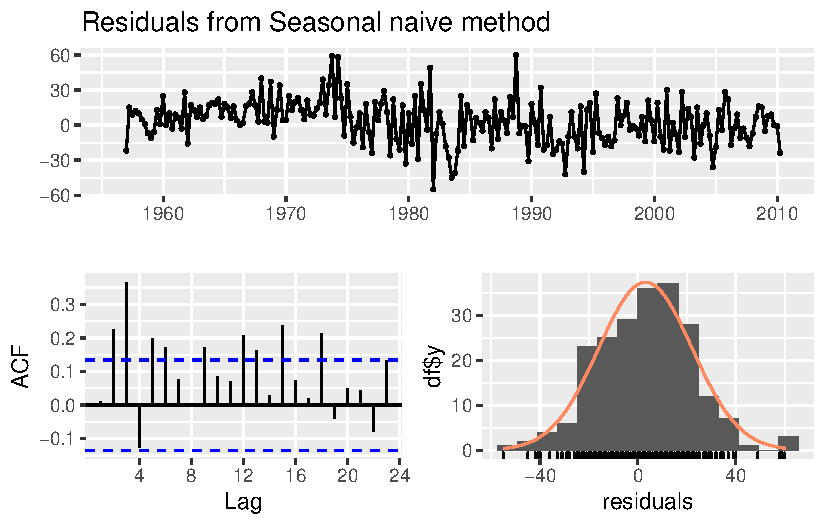
\includegraphics{forecasting_datacamp_ex_files/figure-pdf/unnamed-chunk-8-2.pdf}

}

\end{figure}

\begin{verbatim}

    Ljung-Box test

data:  Residuals from Seasonal naive method
Q* = 60.535, df = 8, p-value = 3.661e-10

Model df: 0.   Total lags used: 8
\end{verbatim}

\begin{Shaded}
\begin{Highlighting}[]
\CommentTok{\# Do they look like white noise (TRUE or FALSE)}
\NormalTok{beerwn }\OtherTok{\textless{}{-}} \ConstantTok{FALSE}
\end{Highlighting}
\end{Shaded}

\hypertarget{evaluating-forecast-accuracy-of-non-seasonal-methods}{%
\subsection{Evaluating forecast accuracy of non-seasonal
methods}\label{evaluating-forecast-accuracy-of-non-seasonal-methods}}

In data science, a training set is a data set that is used to discover
possible relationships. A test set is a data set that is used to verify
the strength of these potential relationships. When you separate a data
set into these parts, you generally allocate more of the data for
training, and less for testing.

One function that can be used to create training and test sets is
subset.ts(), which returns a subset of a time series where the optional
start and end arguments are specified using index values.

\begin{quote}
\hypertarget{x-is-a-numerical-vector-or-time-series}{%
\section{x is a numerical vector or time
series}\label{x-is-a-numerical-vector-or-time-series}}

\hypertarget{to-subset-observations-from-101-to-500}{%
\section{To subset observations from 101 to
500}\label{to-subset-observations-from-101-to-500}}

train \textless- subset(x, start = 101, end = 500, \ldots)
\end{quote}

\begin{quote}
\hypertarget{to-subset-the-first-500-observations}{%
\section{To subset the first 500
observations}\label{to-subset-the-first-500-observations}}

train \textless- subset(x, end = 500, \ldots) As you saw in the video,
another function, accuracy(), computes various forecast accuracy
statistics given the forecasts and the corresponding actual
observations. It is smart enough to find the relevant observations if
you give it more than the ones you are forecasting.
\end{quote}

\begin{quote}
\hypertarget{f-is-an-object-of-class-forecast}{%
\section{f is an object of class
``forecast''}\label{f-is-an-object-of-class-forecast}}

\hypertarget{x-is-a-numerical-vector-or-time-series-1}{%
\section{x is a numerical vector or time
series}\label{x-is-a-numerical-vector-or-time-series-1}}

accuracy(f, x, \ldots) The accuracy measures provided include root mean
squared error (RMSE) which is the square root of the mean squared error
(MSE). Minimizing RMSE, which corresponds with increasing accuracy, is
the same as minimizing MSE.
\end{quote}

The pre-loaded time series gold comprises daily gold prices for 1108
days. Here, you'll use the first 1000 days as a training set, and
compute forecasts for the remaining 108 days. These will be compared to
the actual values for these days using the simple forcasting functions
naive(), which you used earlier in this chapter, and meanf(), which
gives forecasts equal to the mean of all observations. You'll have to
specify the keyword h (which specifies the number of values you want to
forecast) for both.

\hypertarget{instructions-6}{%
\subsubsection{Instructions}\label{instructions-6}}

Use subset() to create a training set for gold comprising the first 1000
observations. This will be called train. Compute forecasts of the test
set, containing the remaining data, using naive() and assign this to
naive\_fc. Set h accordingly. Now, compute forecasts of the same test
set using meanf() and assign this to mean\_fc. Set h accordingly.
Compare the forecast accuracy statistics of the two methods using the
accuracy() function. Based on the above results, store the forecasts
with the higher accuracy as bestforecasts.

\begin{Shaded}
\begin{Highlighting}[]
\CommentTok{\# install.packages("remotes")}
\CommentTok{\#remotes::install\_github("robjhyndman/forecast")}
\FunctionTok{library}\NormalTok{(forecast)}

\CommentTok{\# Create the training data as train}
\NormalTok{train }\OtherTok{\textless{}{-}} \FunctionTok{subset}\NormalTok{(gold, }\AttributeTok{end =} \DecValTok{1000}\NormalTok{)}

\CommentTok{\# Compute naive forecasts and save to naive\_fc}
\NormalTok{naive\_fc }\OtherTok{\textless{}{-}} \FunctionTok{naive}\NormalTok{(train, }\AttributeTok{h =} \DecValTok{108}\NormalTok{)}

\CommentTok{\# Compute mean forecasts and save to mean\_fc}
\NormalTok{mean\_fc }\OtherTok{\textless{}{-}} \FunctionTok{meanf}\NormalTok{(train, }\AttributeTok{h =} \DecValTok{108}\NormalTok{)}

\CommentTok{\# Use accuracy() to compute RMSE statistics}
\CommentTok{\#accuracy(naive\_fc, gold)}
\CommentTok{\#accuracy(mean\_fc, gold)}

\CommentTok{\# Assign one of the two forecasts as bestforecasts}
\NormalTok{bestforecasts }\OtherTok{\textless{}{-}}\NormalTok{ naive\_fc}
\end{Highlighting}
\end{Shaded}

\hypertarget{evaluating-forecast-accuracy-of-seasonal-methods}{%
\subsection{Evaluating forecast accuracy of seasonal
methods}\label{evaluating-forecast-accuracy-of-seasonal-methods}}

As you learned in the first chapter, the window() function specifies the
start and end of a time series using the relevant times rather than the
index values. Either of those two arguments can be formatted as a vector
like c(year, period) which you have also previously used as an argument
for ts(). Again, period refers to quarter here.

Here, you will use the Melbourne quarterly visitor numbers (vn{[},
``Melbourne''{]}) to create three different training sets, omitting the
last 1, 2 and 3 years, respectively. Inspect the pre-loaded vn data in
your console before beginning the exercise; this will help you determine
the correct value to use for the keyword h (which specifies the number
of values you want to forecast) in your forecasting methods.

Then for each training set, compute the next year of data, and finally
compare the mean absolute percentage error (MAPE) of the forecasts using
accuracy(). Why do you think that the MAPE vary so much?

\hypertarget{instructions-7}{%
\subsubsection{Instructions}\label{instructions-7}}

Use window() to create three training sets from vn{[},``Melbourne''{]},
omitting the last 1, 2 and 3 years; call these train1, train2, and
train3, respectively. Set the end keyword accordingly. Compute one year
of forecasts for each training set using the snaive() method. Call these
fc1, fc2, and fc3, respectively. Following the structure of the sample
code, compare the MAPE of the three sets of forecasts using the
accuracy() function as your test set.

\begin{Shaded}
\begin{Highlighting}[]
\CommentTok{\# Create three training series omitting the last 1, 2, and 3 years}
\NormalTok{train1 }\OtherTok{\textless{}{-}} \FunctionTok{window}\NormalTok{(vn[, }\StringTok{"Melbourne"}\NormalTok{], }\AttributeTok{end =} \FunctionTok{c}\NormalTok{(}\DecValTok{2014}\NormalTok{, }\DecValTok{4}\NormalTok{))}
\NormalTok{train2 }\OtherTok{\textless{}{-}} \FunctionTok{window}\NormalTok{(vn[, }\StringTok{"Melbourne"}\NormalTok{], }\AttributeTok{end =} \FunctionTok{c}\NormalTok{(}\DecValTok{2013}\NormalTok{, }\DecValTok{4}\NormalTok{))}
\NormalTok{train3 }\OtherTok{\textless{}{-}} \FunctionTok{window}\NormalTok{(vn[, }\StringTok{"Melbourne"}\NormalTok{], }\AttributeTok{end =} \FunctionTok{c}\NormalTok{(}\DecValTok{2012}\NormalTok{, }\DecValTok{4}\NormalTok{))}

\CommentTok{\# Produce forecasts using snaive()}
\NormalTok{fc1 }\OtherTok{\textless{}{-}} \FunctionTok{snaive}\NormalTok{(train1, }\AttributeTok{h =} \DecValTok{4}\NormalTok{)}
\NormalTok{fc2 }\OtherTok{\textless{}{-}} \FunctionTok{snaive}\NormalTok{(train2, }\AttributeTok{h =} \DecValTok{4}\NormalTok{)}
\NormalTok{fc3 }\OtherTok{\textless{}{-}} \FunctionTok{snaive}\NormalTok{(train3, }\AttributeTok{h =} \DecValTok{4}\NormalTok{)}

\CommentTok{\# Use accuracy() to compare the MAPE of each series}
\CommentTok{\#accuracy(fc1, vn[, "Melbourne"])["Test set", "MAPE"]}
\CommentTok{\#accuracy(fc2, vn[, "Melbourne"])["Test set", "MAPE"]}
\FunctionTok{accuracy}\NormalTok{(fc3, vn[, }\StringTok{"Melbourne"}\NormalTok{])[}\StringTok{"Test set"}\NormalTok{, }\StringTok{"MAPE"}\NormalTok{]}
\end{Highlighting}
\end{Shaded}

\hypertarget{using-tscv-for-time-series-cross-validation}{%
\subsection{Using tsCV() for time series
cross-validation}\label{using-tscv-for-time-series-cross-validation}}

The tsCV() function computes time series cross-validation errors. It
requires you to specify the time series, the forecast method, and the
forecast horizon. Here is the example used in the video:

\begin{quote}
e = tsCV(oil, forecastfunction = naive, h = 1) Here, you will use tsCV()
to compute and plot the MSE values for up to 8 steps ahead, along with
the naive() method applied to the goog data. The exercise uses ggplot2
graphics which you may not be familiar with, but we have provided enough
of the code so you can work out the rest.
\end{quote}

Be sure to reference the slides on tsCV() in the lecture. The goog data
has been loaded into your workspace.

\hypertarget{introduction}{%
\subsubsection{Introduction}\label{introduction}}

Using the goog data and forecasting with the naive() function, compute
the cross-validated errors for up to 8 steps ahead. Assign this to e.
Compute the MSE values for each forecast horizon and remove missing
values in e by specifying the second argument. The expression for
calculating MSE has been provided. Plot the resulting MSE values (y)
against the forecast horizon (x). Think through your knowledge of
functions. If MSE = mse is provided in the list of function arguments,
then mse should refer to an object that exists in your workspace outside
the function, whereas MSE is the variable that you refers to this object
within your function.

\begin{Shaded}
\begin{Highlighting}[]
\CommentTok{\# Compute cross{-}validated errors for up to 8 steps ahead}
\NormalTok{e }\OtherTok{\textless{}{-}} \FunctionTok{tsCV}\NormalTok{(goog, }\AttributeTok{forecastfunction =}\NormalTok{ naive, }\AttributeTok{h =} \DecValTok{8}\NormalTok{)}

\CommentTok{\# Compute the MSE values and remove missing values}
\NormalTok{mse }\OtherTok{\textless{}{-}} \FunctionTok{colMeans}\NormalTok{(e}\SpecialCharTok{\^{}}\DecValTok{2}\NormalTok{, }\AttributeTok{na.rm =} \ConstantTok{TRUE}\NormalTok{)}

\CommentTok{\# Plot the MSE values against the forecast horizon}
\FunctionTok{data.frame}\NormalTok{(}\AttributeTok{h =} \DecValTok{1}\SpecialCharTok{:}\DecValTok{8}\NormalTok{, }\AttributeTok{MSE =}\NormalTok{ mse) }\SpecialCharTok{\%\textgreater{}\%}
  \FunctionTok{ggplot}\NormalTok{(}\FunctionTok{aes}\NormalTok{(}\AttributeTok{x =}\NormalTok{ h, }\AttributeTok{y =}\NormalTok{ MSE)) }\SpecialCharTok{+} \FunctionTok{geom\_point}\NormalTok{()}
\end{Highlighting}
\end{Shaded}

\begin{figure}[H]

{\centering 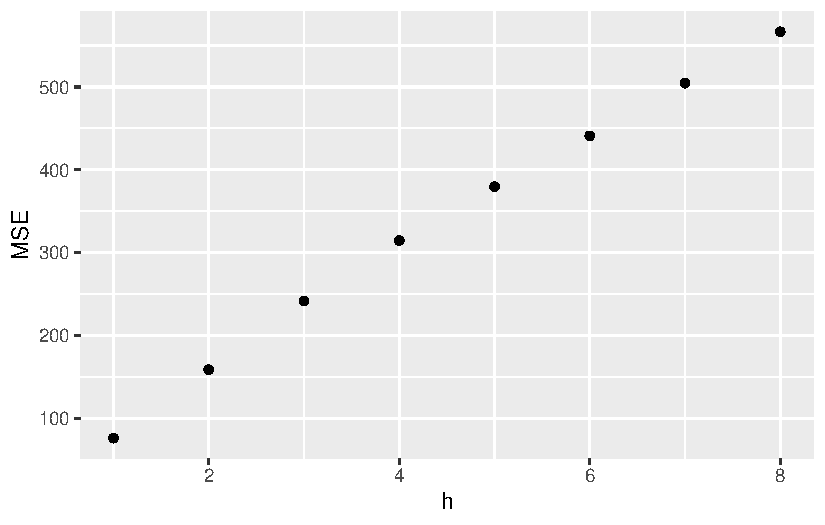
\includegraphics{forecasting_datacamp_ex_files/figure-pdf/unnamed-chunk-11-1.pdf}

}

\end{figure}

\hypertarget{simple-exponential-smoothing}{%
\subsection{Simple exponential
smoothing}\label{simple-exponential-smoothing}}

The ses() function produces forecasts obtained using simple exponential
smoothing (SES). The parameters are estimated using least squares
estimation. All you need to specify is the time series and the forecast
horizon; the default forecast time is h = 10 years.

\begin{quote}
args(ses) function (y, h = 10, \ldots)
\end{quote}

\begin{quote}
fc \textless- ses(oildata, h = 5) summary(fc) You will also use
summary() and fitted(), along with autolayer() for the first time, which
is like autoplot() but it adds a ``layer'' to a plot rather than
creating a new plot.
\end{quote}

Here, you will apply these functions to marathon, the annual winning
times in the Boston marathon from 1897-2016. The data are available in
your workspace.

\hypertarget{instructions-8}{%
\subsubsection{Instructions}\label{instructions-8}}

Use the ses() function to forecast the next 10 years of winning times.
Use the summary() function to see the model parameters and other
information. Use the autoplot() function to plot the forecasts. Add the
one-step forecasts for the training data, or fitted values, to the plot
using fitted() and autolayer().

\begin{Shaded}
\begin{Highlighting}[]
\CommentTok{\# Use ses() to forecast the next 10 years of winning times}
\NormalTok{fc }\OtherTok{\textless{}{-}} \FunctionTok{ses}\NormalTok{(marathon, }\AttributeTok{h =} \DecValTok{10}\NormalTok{)}

\CommentTok{\# Use summary() to see the model parameters}
\FunctionTok{summary}\NormalTok{(fc)}
\end{Highlighting}
\end{Shaded}

\begin{verbatim}

Forecast method: Simple exponential smoothing

Model Information:
Simple exponential smoothing 

Call:
 ses(y = marathon, h = 10) 

  Smoothing parameters:
    alpha = 0.3457 

  Initial states:
    l = 167.1741 

  sigma:  5.519

     AIC     AICc      BIC 
988.4474 988.6543 996.8099 

Error measures:
                     ME     RMSE      MAE        MPE     MAPE      MASE
Training set -0.8874349 5.472771 3.826294 -0.7097395 2.637644 0.8925685
                    ACF1
Training set -0.01211236

Forecasts:
     Point Forecast    Lo 80    Hi 80    Lo 95    Hi 95
2017       130.3563 123.2835 137.4292 119.5394 141.1733
2018       130.3563 122.8727 137.8399 118.9111 141.8015
2019       130.3563 122.4833 138.2293 118.3156 142.3970
2020       130.3563 122.1123 138.6003 117.7482 142.9644
2021       130.3563 121.7573 138.9553 117.2053 143.5074
2022       130.3563 121.4164 139.2963 116.6839 144.0288
2023       130.3563 121.0880 139.6247 116.1816 144.5310
2024       130.3563 120.7708 139.9418 115.6966 145.0161
2025       130.3563 120.4639 140.2488 115.2271 145.4856
2026       130.3563 120.1661 140.5466 114.7717 145.9409
\end{verbatim}

\begin{Shaded}
\begin{Highlighting}[]
\CommentTok{\# Use autoplot() to plot the forecasts}
\FunctionTok{autoplot}\NormalTok{(fc)}
\end{Highlighting}
\end{Shaded}

\begin{figure}[H]

{\centering 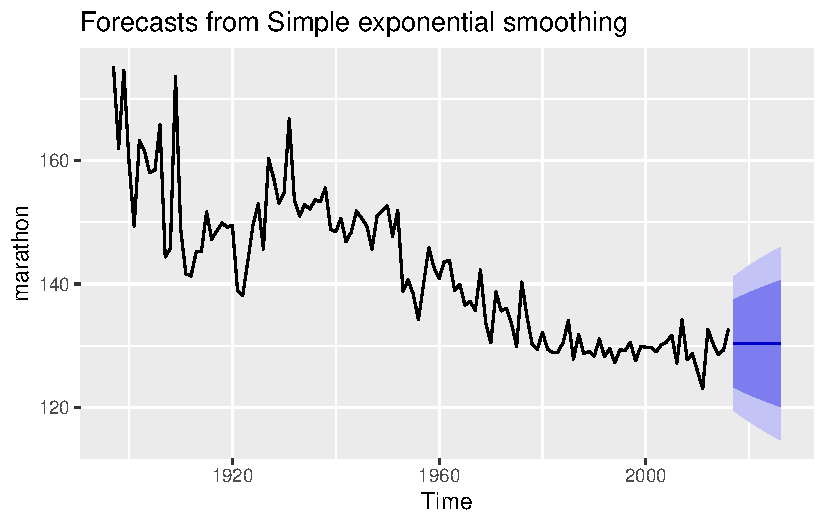
\includegraphics{forecasting_datacamp_ex_files/figure-pdf/unnamed-chunk-12-1.pdf}

}

\end{figure}

\begin{Shaded}
\begin{Highlighting}[]
\CommentTok{\# Add the one{-}step forecasts for the training data to the plot}
\FunctionTok{autoplot}\NormalTok{(fc) }\SpecialCharTok{+} \FunctionTok{autolayer}\NormalTok{(}\FunctionTok{fitted}\NormalTok{(fc))}
\end{Highlighting}
\end{Shaded}

\begin{figure}[H]

{\centering 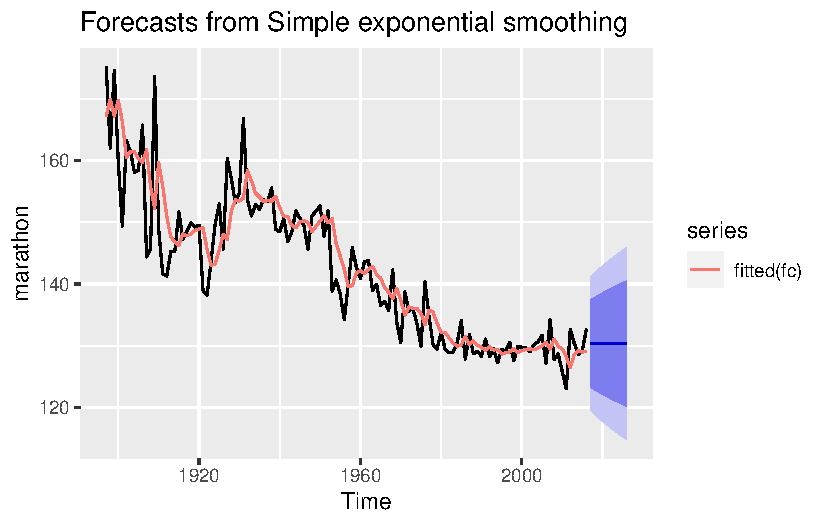
\includegraphics{forecasting_datacamp_ex_files/figure-pdf/unnamed-chunk-12-2.pdf}

}

\end{figure}

\hypertarget{ses-vs-naive}{%
\subsection{SES vs naive}\label{ses-vs-naive}}

In this exercise, you will apply your knowledge of training and test
sets, the subset() function, and the accuracy() function, all of which
you learned in Chapter 2, to compare SES and naive forecasts for the
marathon data.

You did something very similar to compare the naive and mean forecasts
in an earlier exercise ``Evaluating forecast accuracy of non-seasonal
methods''.

Let's review the process:

First, import and load your data. Determine how much of your data you
want to allocate to training, and how much to testing; the sets should
not overlap. Subset the data to create a training set, which you will
use as an argument in your forecasting function(s). Optionally, you can
also create a test set to use later. Compute forecasts of the training
set using whichever forecasting function(s) you choose, and set h equal
to the number of values you want to forecast, which is also the length
of the test set. To view the results, use the accuracy() function with
the forecast as the first argument and original data (or test set) as
the second. Pick a measure in the output, such as RMSE or MAE, to
evaluate the forecast(s); a smaller error indicates higher accuracy. The
marathon data is loaded into your workspace.

\hypertarget{instructions-9}{%
\subsubsection{Instructions}\label{instructions-9}}

Using subset(), create a training set for marathon comprising all but
the last 20 years of the data which you will reserve for testing.
Compute the SES and naive forecasts of this training set and save them
to fcses and fcnaive, respectively. Calculate forecast accuracy measures
of the two sets of forecasts using the accuracy() function in your
console. Assign the best forecasts (either fcses or fcnaive) based on
RMSE to fcbest.

\begin{Shaded}
\begin{Highlighting}[]
\CommentTok{\# Create a training set using subset()}
\NormalTok{train }\OtherTok{\textless{}{-}} \FunctionTok{subset}\NormalTok{(marathon, }\AttributeTok{end =} \FunctionTok{length}\NormalTok{(marathon) }\SpecialCharTok{{-}} \DecValTok{20}\NormalTok{)}

\CommentTok{\# Compute SES and naive forecasts, save to fcses and fcnaive}
\NormalTok{fcses }\OtherTok{\textless{}{-}} \FunctionTok{ses}\NormalTok{(train, }\AttributeTok{h =} \DecValTok{20}\NormalTok{)}
\NormalTok{fcnaive }\OtherTok{\textless{}{-}} \FunctionTok{naive}\NormalTok{(train, }\AttributeTok{h =} \DecValTok{20}\NormalTok{)}

\CommentTok{\# Calculate forecast accuracy measures}
\FunctionTok{accuracy}\NormalTok{( fcses,marathon)}
\end{Highlighting}
\end{Shaded}

\begin{verbatim}
                     ME     RMSE      MAE        MPE     MAPE      MASE
Training set -1.0851741 5.863790 4.155948 -0.8603998 2.827993 0.8990906
Test set      0.4574579 2.493971 1.894237  0.3171919 1.463862 0.4097960
                    ACF1 Theil's U
Training set -0.01595953        NA
Test set     -0.12556096 0.6870735
\end{verbatim}

\begin{Shaded}
\begin{Highlighting}[]
\FunctionTok{accuracy}\NormalTok{(fcnaive, marathon)}
\end{Highlighting}
\end{Shaded}

\begin{verbatim}
                     ME     RMSE      MAE        MPE     MAPE      MASE
Training set -0.4638047 6.904742 4.622391 -0.4086317 3.123559 1.0000000
Test set      0.2266667 2.462113 1.846667  0.1388780 1.429608 0.3995047
                   ACF1 Theil's U
Training set -0.3589323        NA
Test set     -0.1255610 0.6799062
\end{verbatim}

\begin{Shaded}
\begin{Highlighting}[]
\CommentTok{\# Save the best forecasts as fcbest}
\NormalTok{fcbest }\OtherTok{\textless{}{-}}\NormalTok{ fcnaive}
\end{Highlighting}
\end{Shaded}

\hypertarget{holts-trend-methods}{%
\subsection{Holt's trend methods}\label{holts-trend-methods}}

Holt's local trend method is implemented in the holt() function:

\begin{quote}
holt(y, h = 10, \ldots) Here, you will apply it to the austa series,
which contains annual counts of international visitors to Australia from
1980-2015 (in millions). The data has been pre-loaded into your
workspace.
\end{quote}

\hypertarget{instructions-10}{%
\subsubsection{Instructions}\label{instructions-10}}

Produce 10 year forecasts of austa using Holt's method. Set h
accordingly. Use the summary() function to view the model parameters and
other information. Plot your forecasts using the standard time plotting
function. Use checkresiduals() to see if the residuals resemble white
noise.

\begin{Shaded}
\begin{Highlighting}[]
\CommentTok{\# Produce 10 year forecasts of austa using holt()}
\NormalTok{fcholt }\OtherTok{\textless{}{-}} \FunctionTok{holt}\NormalTok{(austa,}\AttributeTok{h=}\DecValTok{10}\NormalTok{)}

\CommentTok{\# Look at fitted model using summary()}
\FunctionTok{summary}\NormalTok{(fcholt)}
\end{Highlighting}
\end{Shaded}

\begin{verbatim}

Forecast method: Holt's method

Model Information:
Holt's method 

Call:
 holt(y = austa, h = 10) 

  Smoothing parameters:
    alpha = 0.9999 
    beta  = 0.0085 

  Initial states:
    l = 0.656 
    b = 0.1706 

  sigma:  0.1952

     AIC     AICc      BIC 
17.14959 19.14959 25.06719 

Error measures:
                     ME      RMSE       MAE       MPE     MAPE      MASE
Training set 0.00372838 0.1840662 0.1611085 -1.222083 5.990319 0.7907078
                  ACF1
Training set 0.2457733

Forecasts:
     Point Forecast    Lo 80    Hi 80    Lo 95    Hi 95
2016       7.030683 6.780483 7.280882 6.648036 7.413330
2017       7.202446 6.847114 7.557778 6.659013 7.745879
2018       7.374209 6.937169 7.811249 6.705814 8.042604
2019       7.545972 7.039179 8.052765 6.770899 8.321045
2020       7.717736 7.148723 8.286748 6.847506 8.587965
2021       7.889499 7.263543 8.515455 6.932181 8.846816
2022       8.061262 7.382302 8.740222 7.022882 9.099642
2023       8.233025 7.504136 8.961915 7.118285 9.347766
2024       8.404788 7.628444 9.181133 7.217472 9.592105
2025       8.576552 7.754792 9.398311 7.319779 9.833324
\end{verbatim}

\begin{Shaded}
\begin{Highlighting}[]
\CommentTok{\# Plot the forecasts}
\FunctionTok{autoplot}\NormalTok{(fcholt)}
\end{Highlighting}
\end{Shaded}

\begin{figure}[H]

{\centering 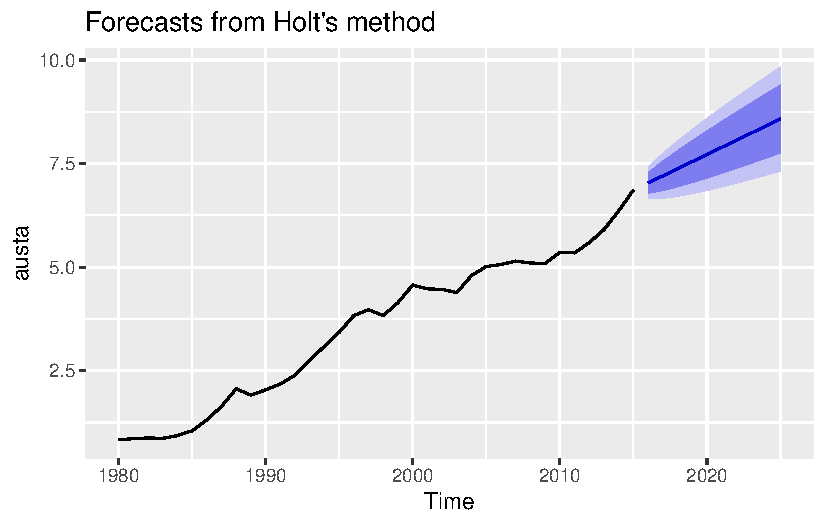
\includegraphics{forecasting_datacamp_ex_files/figure-pdf/unnamed-chunk-14-1.pdf}

}

\end{figure}

\begin{Shaded}
\begin{Highlighting}[]
\CommentTok{\# Check that the residuals look like white noise}
\FunctionTok{checkresiduals}\NormalTok{(fcholt)}
\end{Highlighting}
\end{Shaded}

\begin{figure}[H]

{\centering 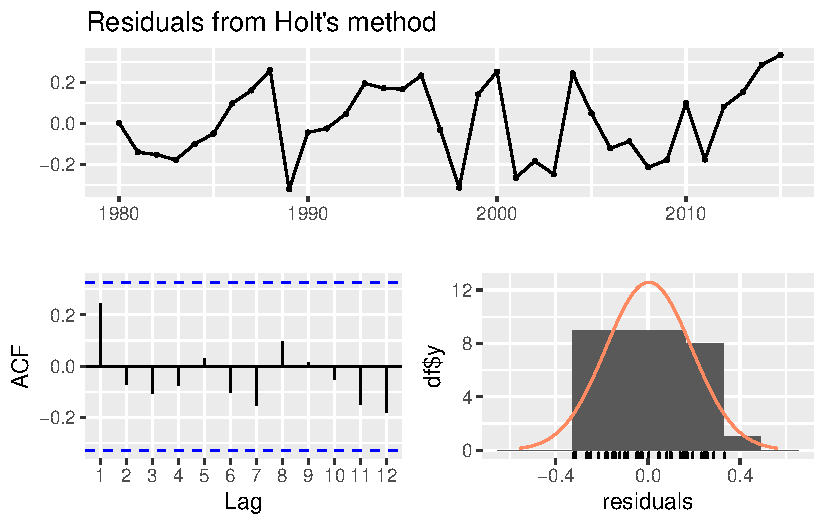
\includegraphics{forecasting_datacamp_ex_files/figure-pdf/unnamed-chunk-14-2.pdf}

}

\end{figure}

\begin{verbatim}

    Ljung-Box test

data:  Residuals from Holt's method
Q* = 4.8886, df = 3, p-value = 0.1801

Model df: 4.   Total lags used: 7
\end{verbatim}

\hypertarget{holt-winters-with-monthly-data}{%
\subsection{Holt-Winters with monthly
data}\label{holt-winters-with-monthly-data}}

In the video, you learned that the hw() function produces forecasts
using the Holt-Winters method specific to whatever you set equal to the
seasonal argument:

fc1 \textless- hw(aust, seasonal = ``additive'') fc2 \textless- hw(aust,
seasonal = ``multiplicative'') Here, you will apply hw() to a10, the
monthly sales of anti-diabetic drugs in Australia from 1991 to 2008. The
data are available in your workspace.

\hypertarget{instructions-11}{%
\subsection{Instructions}\label{instructions-11}}

Produce a time plot of the a10 data. Produce forecasts for the next 3
years using hw() with multiplicative seasonality and save this to fc. Do
the residuals look like white noise? Check them using the appropriate
function and set whitenoise to either TRUE or FALSE. Plot a time plot of
the forecasts.

\hypertarget{solution}{%
\subsubsection{Solution}\label{solution}}

\begin{Shaded}
\begin{Highlighting}[]
\CommentTok{\# Plot the data}
\FunctionTok{autoplot}\NormalTok{(a10)}
\end{Highlighting}
\end{Shaded}

\begin{figure}[H]

{\centering 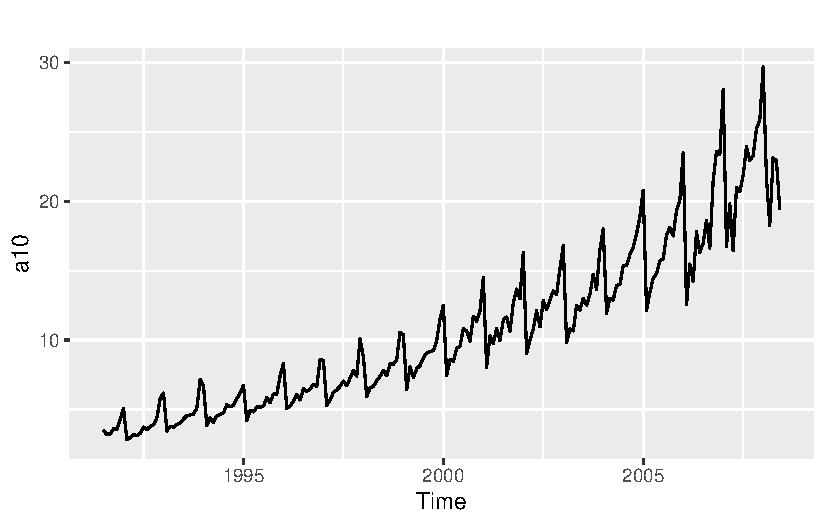
\includegraphics{forecasting_datacamp_ex_files/figure-pdf/unnamed-chunk-16-1.pdf}

}

\end{figure}

\begin{Shaded}
\begin{Highlighting}[]
\CommentTok{\# Produce 3 year forecasts}
\NormalTok{fc }\OtherTok{\textless{}{-}} \FunctionTok{hw}\NormalTok{(a10, }\AttributeTok{seasonal =}\StringTok{"multiplicative"}\NormalTok{, }\AttributeTok{h =} \DecValTok{36}\NormalTok{)}

\CommentTok{\# Check if residuals look like white noise}
\FunctionTok{checkresiduals}\NormalTok{(fc)}
\end{Highlighting}
\end{Shaded}

\begin{figure}[H]

{\centering 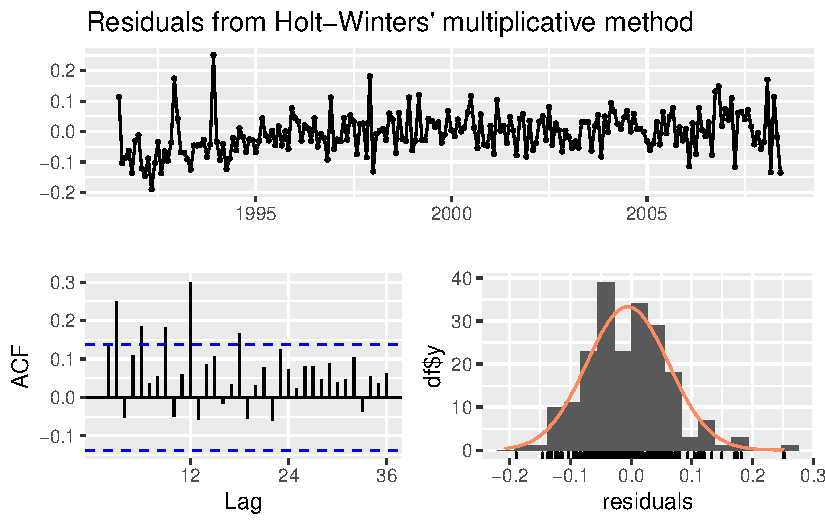
\includegraphics{forecasting_datacamp_ex_files/figure-pdf/unnamed-chunk-16-2.pdf}

}

\end{figure}

\begin{verbatim}

    Ljung-Box test

data:  Residuals from Holt-Winters' multiplicative method
Q* = 75.764, df = 8, p-value = 3.467e-13

Model df: 16.   Total lags used: 24
\end{verbatim}

\begin{Shaded}
\begin{Highlighting}[]
\NormalTok{whitenoise }\OtherTok{\textless{}{-}} \ConstantTok{FALSE}

\CommentTok{\# Plot forecasts}
\FunctionTok{autoplot}\NormalTok{(fc)}
\end{Highlighting}
\end{Shaded}

\begin{figure}[H]

{\centering 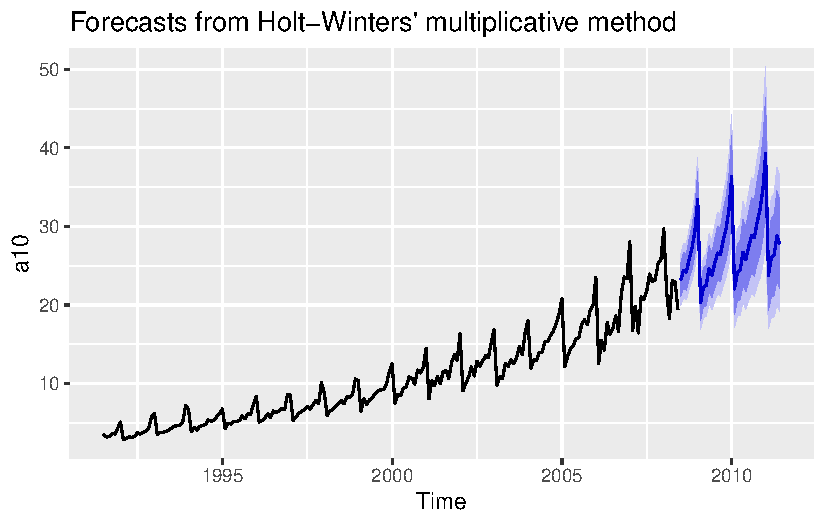
\includegraphics{forecasting_datacamp_ex_files/figure-pdf/unnamed-chunk-16-3.pdf}

}

\end{figure}

\hypertarget{holt-winters-method-with-daily-data}{%
\subsection{Holt-Winters method with daily
data}\label{holt-winters-method-with-daily-data}}

The Holt-Winters method can also be used for daily type of data, where
the seasonal pattern is of length 7, and the appropriate unit of time
for h is in days.

Here, you will compare an additive Holt-Winters method and a seasonal
naive() method for the hyndsight data, which contains the daily
pageviews on the Hyndsight blog for one year starting April 30, 2014.
The data are available in your workspace.

\hypertarget{instructions-12}{%
\subsection{Instructions}\label{instructions-12}}

Using subset.ts(), set up a training set where the last 4 weeks of the
available data in hyndsight have been omitted. Produce forecasts for
these last 4 weeks using hw() and additive seasonality applied to the
training data. Assign this to fchw. Produce seasonal naive forecasts for
the same period. Use the appropriate function, introduced in a previous
chapter, and assign this to fcsn. Which is the better of the two
forecasts based on RMSE? Use the accuracy() function to determine this.
Produce time plots of these forecasts.

\begin{Shaded}
\begin{Highlighting}[]
\CommentTok{\# Create training data with subset()}
\CommentTok{\#train \textless{}{-} subset(\_\_\_, end = \_\_\_)}

\CommentTok{\# Holt{-}Winters additive forecasts as fchw}
\CommentTok{\#fchw \textless{}{-} hw(\_\_\_, seasonal = \_\_\_, h = \_\_\_)}

\CommentTok{\# Seasonal naive forecasts as fcsn}
\CommentTok{\#fcsn \textless{}{-} \_\_\_}

\CommentTok{\# Find better forecasts with accuracy()}
\CommentTok{\#accuracy(\_\_\_, \_\_\_)}
\CommentTok{\#accuracy(\_\_\_, \_\_\_)}

\CommentTok{\# Plot the better forecasts}
\CommentTok{\#autoplot(\_\_\_)}
\end{Highlighting}
\end{Shaded}

\hypertarget{solution-1}{%
\subsubsection{Solution}\label{solution-1}}

\begin{Shaded}
\begin{Highlighting}[]
\CommentTok{\# Create training data with subset()}
\NormalTok{train }\OtherTok{\textless{}{-}} \FunctionTok{subset}\NormalTok{(hyndsight, }\AttributeTok{end =} \FunctionTok{length}\NormalTok{(hyndsight) }\SpecialCharTok{{-}} \DecValTok{28}\NormalTok{)}

\CommentTok{\# Holt{-}Winters additive forecasts as fchw}
\NormalTok{fchw }\OtherTok{\textless{}{-}} \FunctionTok{hw}\NormalTok{(train, }\AttributeTok{seasonal =} \StringTok{"additive"}\NormalTok{, }\AttributeTok{h =} \DecValTok{28}\NormalTok{)}

\CommentTok{\# Seasonal naive forecasts as fcsn}
\NormalTok{fcsn }\OtherTok{\textless{}{-}} \FunctionTok{snaive}\NormalTok{(train, }\AttributeTok{h =} \DecValTok{28}\NormalTok{)}

\CommentTok{\# Find better forecasts with accuracy()}
\FunctionTok{accuracy}\NormalTok{(fchw, hyndsight)}
\end{Highlighting}
\end{Shaded}

\begin{verbatim}
                    ME     RMSE      MAE       MPE    MAPE      MASE      ACF1
Training set -3.976241 228.2440 165.0244 -2.407211 13.9955 0.7492131 0.1900853
Test set     -3.999460 201.7656 152.9584 -3.218292 10.5558 0.6944332 0.3013328
             Theil's U
Training set        NA
Test set     0.4868701
\end{verbatim}

\begin{Shaded}
\begin{Highlighting}[]
\FunctionTok{accuracy}\NormalTok{(fcsn, hyndsight)}
\end{Highlighting}
\end{Shaded}

\begin{verbatim}
                ME     RMSE      MAE        MPE     MAPE      MASE      ACF1
Training set 10.50 310.3282 220.2636 -2.1239387 18.01077 1.0000000 0.4255730
Test set      0.25 202.7610 160.4643 -0.6888732 10.25880 0.7285101 0.3089795
             Theil's U
Training set        NA
Test set      0.450266
\end{verbatim}

\begin{Shaded}
\begin{Highlighting}[]
\CommentTok{\# Plot the better forecasts}
\FunctionTok{autoplot}\NormalTok{(fchw)}
\end{Highlighting}
\end{Shaded}

\begin{figure}[H]

{\centering 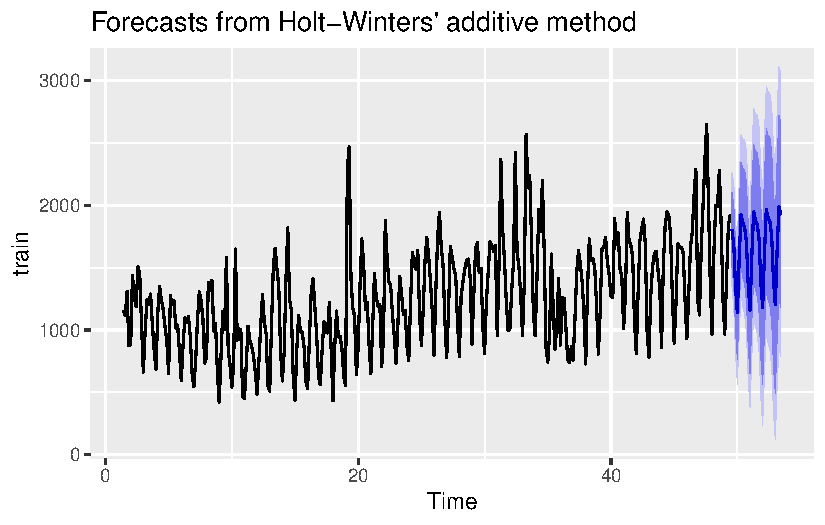
\includegraphics{forecasting_datacamp_ex_files/figure-pdf/unnamed-chunk-18-1.pdf}

}

\end{figure}



\end{document}
